%%%%%%%%%%%%%%%%%%%%%%%%%%%%%%%%%%%%%%%%%%%%%%%%%%%%%%%%%%%%%%%%%%%%%%%%%%%%%%%%
%2345678901234567890123456789012345678901234567890123456789012345678901234567890
%        1         2         3         4         5         6         7         8

%\documentclass[final,letterpaper, 10 pt, conference]{ieeeconf}  % Comment this line out if you need a4paper

%\documentclass[10pt, conference, compsocconf]{IEEEtran}
%\documentclass[a4paper, 10pt, conference]{ieeeconf}      % Use this line for a4 paper
\documentclass[a4paper, 10pt, conference, compsocconf]{ieeeconf}

\IEEEoverridecommandlockouts                              % This command is only needed if
                                                          % you want to use the \thanks command
\pdfminorversion=4
\newcommand{\eu}{\textrm{e}}
\newcommand{\figref}[1]{Fig.~\ref{fig:#1}}
\overrideIEEEmargins
\usepackage[obeyFinal]{todonotes}
\RequirePackage{graphicx}
\usepackage{subfigure}
\usepackage{bm}
%\usepackage{subequation}
\graphicspath{ {figures/} }
\usepackage{url}
%\usepackage{hyperref}
%\usepackage[tight,footnotesize]{subfigure}
\usepackage{fainekos-macros}
\newcommand{\hatodo}[1]{\todo{HA: #1}}
\newcommand{\hatodoin}[1]{\todo[inline]{HA: #1}}
\newcommand{\sAccu}{\epsilon}
\newcommand{\sDelay}{\delta}
\newcommand{\de}{(\sDelay,\sAccu)}
\newcommand{\dek}[1]{(\sDelay_{#1},\sAccu_{#1})}
\newcommand{\hWc}{\widehat{\Wc}}
\newcommand{\sDelayV}{\underline{\sDelay}}
\newcommand{\sAccuV}{\underline{\sAccu}}
\newcommand{\ESet}{\mathcal{E}}
%\newcommand{\bm}{\hat{B}}
\newcommand{\MPCProb}[1]{\mathbb{P_{#1}}}
\newcommand{\RAMPCProb}[2]{\mathbb{P}_{#1}(\hat{\stPt}_{#2},\sDelay_{#2},\sAccu_{#2},\inpPt_{#2 -1})}

% Set macros
%  outer-approximation
\newcommand{\oa}[1]{\mathbf{#1}}
% inner-approximation
\newcommand{\ua}[1]{\underline{#1}}
% make something nominal
\newcommand{\nom}[1]{\bar{#1}}
% in case we use Z somewhere without subscripts
\global\long\def\Zs{Z}
% Zj,k
\newcommand{\Zset}[2]{\Zs_{#1|#2}}
% set for nominal z
\newcommand{\nz}{\nom{z}}
\newcommand{\nomZset}[2]{\overline{Z}_{#1|#2}}
% element nominal z
\newcommand{\nomz}[2]{\nom{z}_{#1|#2}}
% e tilde 
\newcommand{\te}{\tilde{e}}
% set E tilde
\newcommand{\tE}{\widetilde{E}}
% w hat,x hat
\newcommand{\hw}{\widehat{w}}
% W hat set
\newcommand{\What}{\widehat{W}}
% z hat
\newcommand{\hz}{\hat{z}}
% x hat, X set
\newcommand{\hx}{\hat{x}}
\newcommand{\Xset}[2]{X_{#1|#2}}
\newcommand{\oaXset}[2]{\oa{X}_{#1|#2}}
% reach set
\newcommand{\RT}[1]{RT_{=T}(#1,U)}
% T inverse
\newcommand{\iT}{T^{-1}}
% Problem
\newcommand{\Pk}[1]{\mathbb{P}_{#1}(\hat{z}_{#1})}


\newcommand{\such}{\;|\;}
% Dimensions
\global\long\def\dimX{n_x}
\global\long\def\dimZ{n_z}
\global\long\def\dimV{n_v}
\global\long\def\dimU{n_u}

\global\long\def\Cc{\mathcal{C}}
\newboolean{TECH_REPORT}
\setboolean{TECH_REPORT}{FALSE}


\newtheorem{theorem}{Theorem}
\newtheorem{corollary}{Corollary}[theorem]
\newtheorem{lemma}[theorem]{Lemma}

\usepackage{array}
\usepackage{url}
\usepackage{gensymb}

\usepackage{algpseudocode}  % Of the algorithmicx package, flexible, more math-like
\usepackage{algorithm}


\newcommand\Mark[1]{\textsuperscript#1}

% See the \addtolength command later in the file to balance the column lengths
% on the last page of the document

% The following packages can be found on http:\\www.ctan.org
%\usepackage{graphics} % for pdf, bitmapped graphics files
%\usepackage{epsfig} % for postscript graphics files
%\usepackage{mathptmx} % assumes new font selection scheme installed
%\usepackage{times} % assumes new font selection scheme installed
\usepackage{amsmath} % assumes amsmath package installed
\usepackage{amssymb}  % assumes amsmath package installed

\title{
Robust Model Predictive Control for Non-Linear Systems with Input and State Constraints Via Feedback Linearization
}
%
\author{Yash Vardhan Pant, Houssam Abbas, Rahul Mangharam% <-this % stops a space
\thanks{*This work was supported by STARnet a Semiconductor Research
Corporation program sponsored by MARCO and DARPA, NSF MRI-0923518 and the US Department of Transportation University Transportation Center Program}% <-this % stops a space
\thanks{The Departments of Electrical and Systems Engineering and Computer and Information Sciences, University of Pennsylvania, Philadelphia, U.S.A.
        {\small
        \{yashpant,habbas,rahulm\}@seas.upenn.edu}}%
}





\begin{document}

\maketitle
\thispagestyle{empty}
\pagestyle{empty}

\begin{abstract}
 
 
 
 
 Cyber-Physical Systems must withstand a wide range of errors, from bugs in their software to attacks on their physical sensors.
 Given a formal specification of their desired behavior in Metric Temporal Logic (MTL), the robust semantics of the specification provides a notion of \textit{system robustness} that can be calculated directly on the output behavior of the system, without explicit reference to the various sources or models of the errors.
 The robustness of the MTL specification has been used both to verify the system offline (via robustness minimization) and to control the system online (to maximize its robustness over some horizon).
 Unfortunately, the robustness objective function is difficult to work with: it is recursively defined, non-convex and non-differentiable.
 In this paper, we propose smooth approximations of the robustness. 
 Such approximations are differentiable, thus enabling us to use powerful off-the-shelf gradient descent algorithms for optimizing it.
 By using them we can also offer guarantees on the performance of the optimization in terms of convergence to minima.
 We show that the approximation error is bounded to any desired level, and that the approximation can be tuned to the specification.
 We demonstrate the use of the smooth robustness to control two quad-rotors in an autonomous air traffic control scenario, and for temperature control of a building for comfort.
\end{abstract}

\section{Introduction}
\label{sec:intro}

New:
nonlinear control with mpc on feedback linearized dynamics with state estimation error, input constraints, state constraints
	feedback linearization but no state constraints and identity T, no state uncertainty
	
state constraints
recursive feasibility with time-varying error sets

\textbf{Notation}.
Given two subsets $A,B$ of $\Re^n$, define their \textit{Minkowski sum} to be $A\oplus B \defeq \{a+b \such a\in A, b\in B\}$.
Define their Pontryagin difference to be $A\ominus B = \{c \in \Re^n \such c+b \in A \forall b \in B\}$
\section{Problem Formulation} \label{sec:formulation}

The control problem is as follows:

\begin{subequations}
\begin{align}
\text{Minimize } &l(x,u) \\
&\text{s.t.} \nonumber \\
\dot{x}&=f(x)+G(x)u \\
x&\in X\\
u&\in U
\end{align}
\end{subequations}

A discrete-time, periodic, state-estimator provides access to a state estimate with estimation error
\begin{subequations}
\begin{align}
\hat{x}(t)&=x(t)+e(t) \\ 
\text{where, } e(t) &\in E
\end{align}
\end{subequations}

\section{Robust MPC for the feedback linearized system}

Following \cite{RichardsH05_RMPC}, \cite{PantAMNDM15_Anytime}, we formulate a Robust MPC (RMPC) controller of \eqref{eq:discrete linear problem} via \emph{constraint restriction}.
We outline the idea before providing the technical details.
The key idea is to move the effects of estimation error $\tilde{e}_k$ and  process noise $w_k$ (the `disturbances') to the constraints, and work with the nominal  (i.e., disturbance-free) dynamics: $\nz_{k+1} = A\nz_{k}+Bv_k$, $\nz_{0} = z_0$.
Because we would be optimizing over disturbance-free states, we must account for the noise in the constraints. 
Specifically, rather than require the next (nominal) state $\nz_{k+1}$ to be in $Z$, we require it to be in the shrunk set $Z \ominus \What_{k+1|k} \ominus \tE_{k+1|k}$: by definition of Pontryagin difference, this implies that whatever the actual value of the noise $\hw_{k+1} \in \What_{k+1|k}$ and of the estimation error $\tilde{e}_{k+1} \in \tE_{k+1|k}$, the actual state $z_{k+1}$ will be in $Z$. 
This is repeated over the entire MPC prediction horizon $j=1,\ldots,N$, with further shrinking at every step.
For further steps ($j>1$), the process noise $\What_{k+j|k}$ is propagated through the dynamics, so the shrinking term $\What$ is shaped by a stabilizing feedback controller $x \mapsto Kx$.
At the final step ($j=N$), a terminal constraint is derived using the worst case estimation error set $\tE_{max}$ and a convex global inner approximation for the input constraints, $V_{inner-global}$. 
Details of this construction follow below.

Through this successive constraint tightening we ensure robust safety and feasibility of the feedback linearized system (and hence of the non-linear system). 
Since we use just the nominal dynamics, and show that the tightened constraints are linear in the state and inputs, we still solve a Quadratic Program (QP) for the MPC optimization.
The difficulty of applying RMPC in our setting is that the amounts by which the various sets are shrunk varies with time and is (nonlinear) state-dependent, and involves set computations with the non-convexity preserving mapping $T$.
One of our contributions in this paper is to establish recursive feasibility of MPC with time-varying constraint sets.
% This not only allows us to keep a check on the complexity of the MPC optimization, but also allows us to formulate the MPC with a quadratic cost on the input to the feedback linearized system \textbf{[InputPaperRef8]}.

%
%\textbf{Note:} So far we have not found an expression for the bound on $\tilde{e}_k$ given $e_k \in E$. While for the rest of this section we assume we have a polyhedral bound $\tilde{e}_k \in \tilde{E}_k \, \forall k$, we will show how to explicitly compute this bounding set $\tilde{E}_k$ using online reachability in Sec.?? . Since we compute $\tilde{E}_{k+j},\, j\geq 0$ using an online reachability method that depends on the state estimate at time $k$, we represent the set as $\tilde{E}_{k+j|k}$ to explicitly show its dependence on the state estimate at time $k$. Similarly, the computed bound for $\What_{k+1}$, given state estimate at time $k$, is given by $\What_{k+1|k}=W\oplus{E}_{k+1|k}\oplus(-A\tilde{E_{k|k}})$. 


\todo[inline]{mention that if shrunk terminal set is non-empty, then nothing in between is empty. }
The RMPC optimization  $\mathbb{P}_{k_0}(\hat{z}_{k_0})$ for solving \eqref{eq:discrete linear problem} is:
%\begin{eqnarray} 
%	\label{eq:nom mpc}
%	J^{*}(\nz_{k}) &=& \min_{\mathbf{\nz},\mathbf{u}} \sum_{j=0}^{N}\lbrace \nz_{k+j|k}^{T}Q \nz_{k+j|k} + {v}_{k+j|k}^{T}R{v}_{k+j|k}\rbrace \nonumber \\ 
%	&\quad & +  \nz_{k+N+1|k}^T Q_f \nz_{k+N+1|k}  \label{eq:cost} \\
%	\nz_{k|k}       &= &\hat{z}_{k} \label{eq:init_cond}\\
%	\nz_{k+j+1|k} &=&A\nz_{k+j|k} + Bv_{k+j|k} , j=0,\ldots,N\label{eq:nom_dyn} \\
%	\nz_{k+j|k}     & \in& \nomZset{k+j}{k} , \; j=0,\ldots,N \label{eq:states_con}\\
%	v_{k+j|k}        & \in & V_{k+j|k} , \;j=0,\ldots,N-1 \label{eq:input_con} \\
%	p_N               &= &\lbrack z_{k+N+1|k} , v_{k+N|k} \rbrack^{T}  \in P_f \label{eq:joint_term} 
%\end{eqnarray}
\begin{subequations} 
\label{eq:nom mpc}
\begin{align}
J^{*}(\nz_{k}) &= \min_{\mathbf{\nz},\mathbf{u}} \sum_{j=0}^{N}\lbrace \nz_{k+j|k}^{T}Q \nz_{k+j|k} + {v}_{k+j|k}^{T}R{v}_{k+j|k}\rbrace \nonumber \\ 
                    &\quad  +  \nz_{k+N+1|k}^T Q_f \nz_{k+N+1|k}  \label{eq:cost} \\
\nz_{k|k}       &= \hat{z}_{k} \label{eq:init_cond}\\
\nz_{k+j+1|k} &=A\nz_{k+j|k} + Bv_{k+j|k} , j=0,\ldots,N\label{eq:nom_dyn} \\
\nz_{k+j|k}     & \in \nomZset{k+j}{k} , \; j=0,\ldots,N \label{eq:states_con}\\
v_{k+j|k}        & \in  V_{k+j|k} , \;j=0,\ldots,N-1 \label{eq:input_con} \\
p_{N+1}               &= \lbrack z_{k+N+1|k} , v_{k+N|k} \rbrack^{T}  \in P_f \label{eq:joint_term} 
	\end{align}
\end{subequations}

Here, $\nz$ is the state of the nominal linearized system
The cost and constraints of the optimization are explained below:
\begin{itemize}
\item Eq. \eqref{eq:cost} shows a cost quadratic in $\nz$ and $v$, where as usual $Q$ is positive definite and R is positive semi-definite. 
In the terminal cost term, $Q_f$ is the solution of the Lyapunov equation $Q_f-(A+BK)^{T}Q_f(A+BK) = Q+K^{T}RK$.
This choice guarantees that the terminal cost equals the infinite horizon cost under a linear feedback control $\nz \mapsto K\nz$ \cite{CannonK15MPC}.

\item Eq. \eqref{eq:nom_dyn} gives the nominal dynamics of the discretized linearized system.

\item Eq. \eqref{eq:init_cond} initializes the nominal state with the current state estimate.

\item Eq. \eqref{eq:states_con} tightens the admissible set of the nominal state by a sequence of shrinking sets.

\item Eq. \eqref{eq:input_con} constrains $v_{k+j|k}$ such that the corresponding $u(x,v)$ is admissible, and the MPC is recursively feasible.

\item Eq. \eqref{eq:joint_term} constrains the final input and nominal state to be within a terminal set $P_f$.

\end{itemize}

\subsection{State and Input Constraints for the Robust MPC}
\label{sec:Constraints}
The state and input constraints for the RMPC are defined as follows:

\textit{The state constraints $\nomZset{k+j}{k}$:}
The tightened state constraints are functions of the error sets $\tE_{k+j|k}$ and disturbance sets $What_{k+j|k}$, and defined $\forall\,j=0,\dotsc,N$
{\small{
\begin{equation} 
\label{eq:Set_constraints}
\nomZset{k+j}{k} = Z \ominus_{i=0}^{j-1}(L_i \What_{k+(j-i)|k})\ominus (-\tE_{k+j|k})
\end{equation}
}}
(Recall $Z$ is a subset of $T(X)$, $\What_{k+j|k}$ and $\tE_{k+j|k}$ are formally defined in Sec. \ref{sec:set definitions}).
The state transition matrix $L_j$, $\forall j=0,\dotsc,N$   is defined as $L_0 = \mathbb{I}, L_{j+1} = (A+BK)L_j $.
The intuition behind this construction was given at the start of this section.

\textit{The input constraints $V_{k+j|k}$:}
$\forall j=0,...,N-1$
\begin{equation} 
\label{eq:input_constraints}
V_{k+j|k} = \ua{V}_{k+j|k} \ominus_{i=0}^{j-1}KL_i\What_{k+(j-i)|k} 
\end{equation}
where $\ua{V}_{k+j|k} $ is an inner-approximation of the set of admissible inputs $v$ at prediction step $j+k|k$, as defined in Sec. \ref{sec:approx input sets}.
The intuition behind this construction is similar to that of $\nomZset{k+j}{j}$: given the inner approximation $\ua{V}_{k|k} $, it is further shrunk at each prediction step $j$ by propagating forward the noise $\hw_k$ through the dynamics, and shaped according to the stabilizing feedback law $K$, following \cite{RichardsH05_RMPC}.

\textit{The terminal constraint $P_f$:}
This constrains the extended state $p_k = [\nz_{k}, v_{k-1}]^T$, and is given by 
\begin{equation}
\label{eq:P_f_def}
P_f = C_p\ominus \left\lbrack \begin{matrix} (A+BK)^N \\ K(A+BK)^{N-1}\end{matrix} \right \rbrack \What_{max}
\end{equation}
where $\What_{max} \subset \Re^{\dimZ}$ is a bounding set on the worst-case disturbance (we show how it's computed in Sec. \ref{sec:approx dist}),
and $C_p \subset \Re^{\dimZ}\times \Re^{\dimV}$ is an invariant set of the nominal dynamics subject to the stabilizing controller $\nz \mapsto K\nz$, naturally extended to the extended state $p$:
that is, there exists a feedback control law $p \mapsto \widehat{K}p$, such that $\forall p\in C_p$
\begin{eqnarray}
\label{eq:C_def}
\widehat{A} p + \widehat{B} \widehat{K} p + \widehat{L}_N  [\hw^T, 0^T]^T \, \in C_p,\, \forall \hw \in \What_{max} 
\end{eqnarray}
with $\widehat{A} = \begin{bmatrix} A & 0_{n \times m} \\ 0_{m \times n} & 0_{m \times m}   \end{bmatrix} $,
$\widehat{B} = \begin{bmatrix}  B \\ \mathbb{I}_{m \times m} \end{bmatrix}$, 
$\widehat{K} = \begin{bmatrix}  K & 0_{m \times m}  \end{bmatrix}$,
$\widehat{L} _N = (\widehat{A} + \widehat{B} \widehat{K})^N$.
It is important to note the following:
\begin{itemize}
	\item The set $P_f$ can be computed offline since it depends on $\What_{max}$, $\tE_{max}$ and the global inner approximation for the constraints on $v$, $V_{inner-global}$, all of which can be computed offline.
	\item If $P_f$ is non-empty, then all intermediate sets that appear in \eqref{eq:nom mpc} are also non-empty, since $P_f$ shrinks the state and input sets by the maximum disturbances $\What_{max}$ and $\tE_{max}$.	
	Thus we can tell, before running the system, whether RMPC might be faced with empty constraint sets (and thus infeasible optimizations).
	\item Note that all constraints are linear.x
\end{itemize}




\subsection{Robust Feasibility}

The Robust MPC algorithm, with its constraints and the error set computations for bounding $\tilde{e}_k$ using online reachability, is designed to be robustly feasible to the estimation error, $e_k$, in the estimate of the non-linear system $\hat{x}_k$. This is stated in Theorem \ref{th:robust_feas}, which follows.

\begin{theorem}
\label{th:robust_feas}
If for some time step $k_0$, the Robust MPC optimization, $\mathbb{P}_{k_0}(\hat{z}_{k_0})$ is feasible, then the feedback linearized system, and hence the non-linear system controlled by the Robust MPC of algorithm \textbf{algref} and subject to the disturbances (\textbf{esterror,processnoise}) robutly satisfies the state and input constraints \textbf{eqns} and all subsequent optimizations $\mathbb{P}_{k}(\hat{z}_{k}), \, \forall k>k_0$ are feasible.
\end{theorem}

With this result, the proof of which is in the \textbf{Appendix}, we can state Theorem \ref{th:recursive_feas}.

\begin{theorem}
\label{th:recursive_feas}
If at the initial time step, $\mathbb{P}_0(\hat{z}_0)$ is feasible, then the the feedback linearized, and hence the non-linear system, subject to the disturbances  (\textbf{esterror,processnoise}) satisfies the state and input constraints under the control law of \textbf{algref}, and all subsequent iterations of the algorithm are feasible.
\end{theorem}

\begin{proof}
The Theorem can be proved recursively by applying Theorem \ref{th:robust_feas}. Suppose at time step $k$, the algorithm is feasible and the control input computed by it is $v_k$, by Theorem \ref{th:robust_feas}, $v_k$ is feasible and so $u_k \in U$. Under this control input, the state at time $k+1$, $z_{k+1} \in Z$, and $\mathbb{P}_{k+1}(\hat{x}_{k+1})$ is also feasible, i.e. the algorithm is feasible. Therefore, by induction, the Theorem holds. 
\end{proof}


\begin{theorem}[Stability]
%	\label{thm:stability}
%Given an equilibrium point $x_e \in X_0 \subset \iT(Z)$ of the nonlinear dynamics \eqref{eq:generic NLMPC}, Algorithm \ref{alg:RMPC} stabilizes the nonlinear system to $x_e$.
%\end{theorem}
	\label{thm:stability}
Given an equilibrium point $x_e \in X_0 \subset \iT(Z)$ of the nonlinear dynamics \eqref{eq:generic NLMPC}, Algorithm \ref{alg:RMPC} stabilizes the nonlinear system to an invariant set around $x_e$.
\end{theorem}

\begin{proof}
Let $T$ be the diffeomorphism mapping $x$ to $z$ from feedback linearization.
By a change of variables $z' = z - T(x_e)$, stabilizing the linear dynamics (with state $z'$) to 0 implies stabilizing the nonlinear dynamics to $x_e$.
Recall that $Q$ and $Q_f$ of  \eqref{eq:nom mpc} are positive definite and that $R$ is positive semi-definite,  so that the optimal cost $J^*(\nz_{k})$ is a positive definite function of $\nz_{k}$, and that the terminal weight in \eqref{eq:nom mpc} is equivalent to the infinite horizon cost (by our choice of $Q_f$). 
Finally Thm.  \ref{th:robust_feas} guarantees that the tail of the input sequence computed at $k$ is admissible at time $k+1$. 
Therefore it is a standard result that the optimal cost $J^{*}({\nz}_{k})$ is non-increasing in $k$ and that $0$ is a stable equilibrium for the closed-loop linear system (e.g., see \cite{CannonK15MPC} ). 
Moreover the nominal feedback-linearized system ($\nz$) converges to 0 from anywhere in $Z$. Therefore, the nominal $\bar{x}_{k}$ converges to $x_e$ from anywhere in $X_0 \subset \iT(Z)$. The true state ($x_k$) then converges to the invariant set around $x_e$.
\end{proof}
\section{Set definitions for the RMPC}

Algorithm \ref{alg:RMPC} and the problem $\Pk{k}$ \eqref{eq:nom mpc} use a number of constraint sets to ensure recursive feasibility of the successive RMPC optimizations, namely: 
inner approximations of the admissible input sets $\ua{V}_{k+j|k}$, 
bounding sets for the ($T$-mapped) estimation error $\tE_{k+j|k}$, 
bounding sets for the process noise $\What_{k+j|k}$, 
and the largest error and noise sets $\tE_{max}$ and $\What_{max}$.
In this section we show how these sets are defined and computed.

 \subsection{Over-approximating the reach set of the nonlinear system}
\label{sec:x reach}

At time $k$, we need to compute the forward reach set, starting from $x_k$, for the next $N$ steps, for two purposes:
first, this is needed for defining the constraints on the input $v$ to the linearized dynamics.
Secondly, this is needed to compute a containing set for the estimation error in $z$-space.

In all but the simplest systems, forward reachable sets can not be computed exactly.
Moreover, the true state $x_k$ is not known.
Therefore we show how to compute an outer-approximation $\oaXset{k+j}{k},  j=0,\ldots, N$.
To do so we may use a reachability tool for nonlinear systems, RTreach??. 
A reachability tool computes an outer-approximation of the reachable set of a system starting from some set $\Xc \subset X$, subjet to inputs from a set $U$, for a duration $T \geq 0$. 
Denote this approximation by $\RT{\Xc}$.

At time $k$, the state estimate $\hx_{k}$ is known.
Therefore $x_k = \hx_{k} - e_k \in \hx_{k} \oplus (-E) \defeq \Xset{k}{k}$.
Propagating $\Xset{k}{k}$ forward one step through the continuous-time nonlinear dynamics yields $\Xset{k+1}{k}$, which is outer-approximated by $\RT{\Xset{k}{k}}$.
The estimate that the system will receive at time $k+1$ is therefore bound to be in the set $\RT{\Xset{k}{k}}  \oplus E$.
Since $0 \in E$, we maintain $\Xset{k+1}{k} \subset \RT{\Xset{k}{k}}  \oplus E$.
We define the over-approximate reach set at $k+1$, computed at time $k$, to be 
\begin{equation*}
\label{eq:def Xk}
\oaXset{k+1}{k} \defeq  \RT{\Xset{k}{k}}  \oplus E \oplus  (-E)
\end{equation*}
%(The reason for adding the extra $-E$ term will be apparent in the proof to Thm.??).
Fig. \ref{fig:overreach_NL} shows a visualization of this approach.

More generally, for $1 \leq j \leq N$, we define the $j$-step reach set computed at time $k$ to be
\begin{eqnarray}
\label{eq:def Xkj}
\oaXset{k}{k} &\defeq&   \hx_{k} \oplus (-E) 
\nonumber
\\
\oaXset{k+j}{k} & \defeq& \RT{\oaXset{k+j-1}{k}} \oplus E \oplus (-E) 
\end{eqnarray}

The following holds by construction:
\begin{lemma}
	\label{lemma:xreach}
	For any time $k$ and step $j \geq 1$, the $j$-step reach set of the non-linear dynamics starting from $x_k$ is outer-approximated by $\oaXset{k+j}{k}$:
	$\Xset{k+j}{k} \subset \oaXset{k+j}{k}$.
\end{lemma}


\begin{figure*}
\includegraphics[scale=0.75]{figs/OverReachFigure_NL_scissored.pdf}
\caption{The over-approximated reachable sets for $x_{k+j}$, computed at time steps $k$, and correspondingly ay $k+1$ , used to compute $\tilde{E}_{k+j|k}$, $\underline{V}_{k+j|k}$. }
\label{fig:overreach_NL}
\end{figure*}

This construction of the outer-approximation permits us to prove recursive feasibility of the MPC controller,  because it causes the constraints of the MPC problem setup at time $k+1$ to be consistent with (stronger than) the constraints of the MPC problem setup at time $k$.
This will be explicitly stated and proved in the proof of Thm. ??

\subsection{Approximating the bounding sets for the input}
\label{sec:approx input sets}
Given $x \in X$, define the set $V(x) \defeq \{v \in \Re^{\dimV} \such u(x) = R^{-1}(x)[b(x)+v] \in U\}$.
We assume that there exist functions $\ua{v}_i, \oa{v}_i: X \rightarrow \Re$ s.t. for any $x$, $V(x) = \{[v_1,\ldots,v_{\dimV}]^T \such \ua{v}_i(x) \leq v_i \leq \oa{v_i}(x) \}$.
Because in general $V(x)$ is not a rectangle, we work with inner and outer rectangular approximations of $V(x)$.
Specifically, let $\Xc$ be a subset of $X$.
Define the inner and outer bounding rectangles, respectively
\[\ua{V}(\Xc) \defeq \{v=[v_1,\ldots,v_{\dimV}]^T \such \max_{x\in \Xc} \ua{v}_i(x)  \leq v_i \leq \min_{x \in \Xc} \oa{v}_i(x) \} \]
\[\oa{V}(\Xc) \defeq \{v=[v_1,\ldots,v_{\dimV}]^T \such \min_{x\in \Xc} \ua{v}_i(x)  \leq v_i \leq \max_{x \in \Xc} \oa{v}_i(x) \} \]

By construction, we have for any subset $\Xc \subset X$
\begin{equation}
\label{eq:Vbounds}
\ua{V}(\Xc) \leq \cup_{x \in \Xc} V(x) \subset \oa{V}(\Xc)
\end{equation}
If two subsets of $X$ satisfy $\Xc_1 \subset \Xc_2$, then it holds that 
\begin{equation}
\label{eq:V inclusions}
\ua{V}(\Xc_2) \subset \ua{V}(\Xc_1), \; \oa{V}(\Xc_1) \subset \oa{V}(\Xc_2)
\end{equation}

Using the reachability over-approximations of Sec. \ref{sec:x reach} we can compute:
\begin{equation}
\label{eq:Vkj Vmax}
\ua{V}_{k+j|k}  = \ua{V}(\oa{X}_{k+j|k}), \; \ua{V}_{inner-global} = \ua{V}(X)
\end{equation}
In practice we use interval arithmetic to compute these sets since $\oaXset{k+j}{k}$ and $U$ are hyper-intervals.

\begin{figure}
	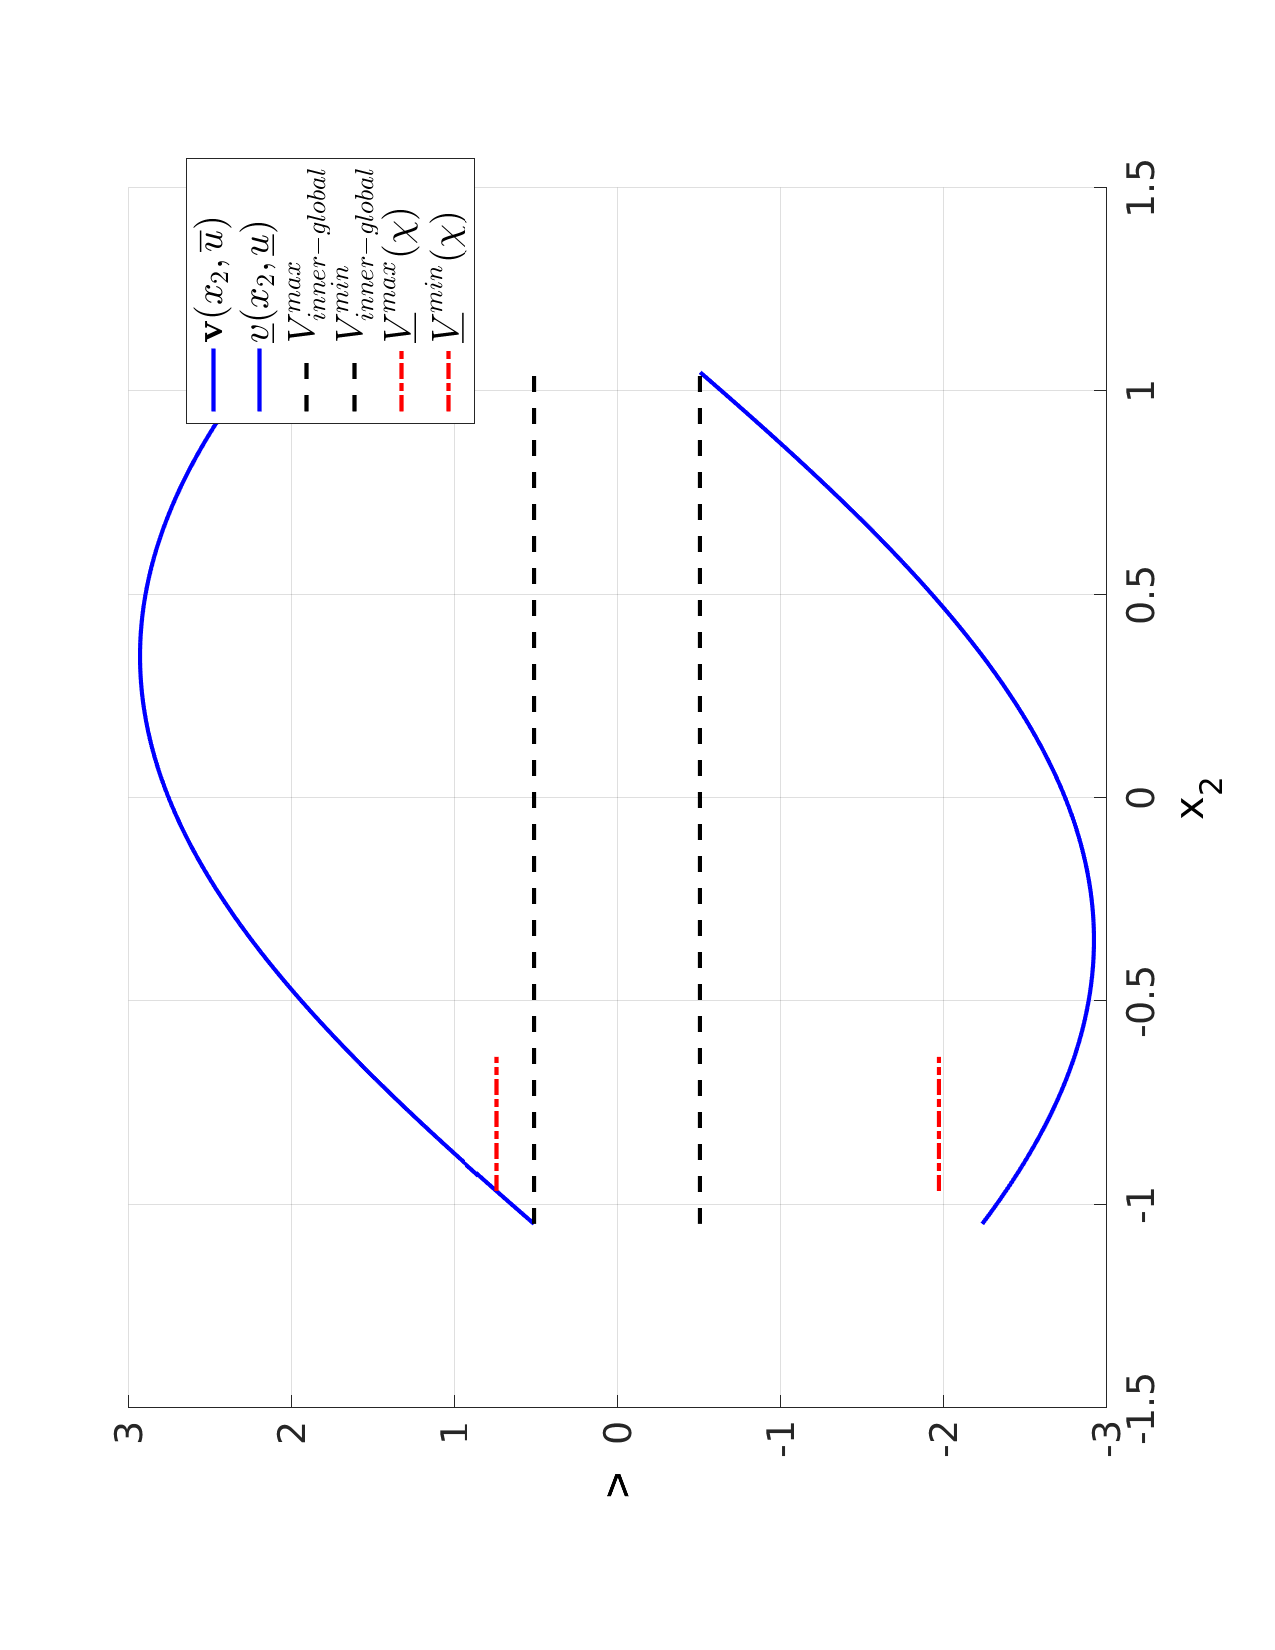
\includegraphics[angle=270,width=0.49\textwidth]{figs/InputToy.pdf}
	\caption{The local (over $\Xc$) and global (over $X$) inner approximations of input constraints for running example, with $\Xc =  [-\pi/4,0]\times[-0.9666,-0.6283]$ and $U = [-2.75,2.75]$.}
	\label{fig:err bounds toy}
\end{figure}

Fig. \ref{fig:err bounds toy} shows these sets for the running example.



\subsection{Approximating the bounding sets for the disturbances}
\label{sec:approx dist}
We will also need to define containing sets for the state estimation error in $z$ space:
recall that $\hat{z}_k = T(\hat{x}_k) = T(x_k+e_k)$. 
%******************
We use a Taylor expansion
\begin{eqnarray}
\label{eq:taylor expansion T}
\hat{z}_k &=& T(x_k) + \underbrace{\frac{dT}{dx}(x_k)}_{M(x_k)}e_k+ \underbrace{\frac{1}{2}e_k^T \frac{d^2T}{dx^2}(c)e_k}_{r_k(c)}, c \in x_k + E \nonumber 
\\
&=& T(x_k) + M(x_k)e_k+ r_k(c), c \in x_k + E \nonumber
\\
&=& T(x_k) + \te_{k}+ r_k(c), c \in x_k + E \nonumber
\end{eqnarray}

The remainder term $r_k(c)$ is bounded in the set $R_k = \cup_{c \in \hx_{k}-e +E}   (1/2)e^T\frac{d^2T}{dx^2}(c)e_k$
%******************
We assume that the magnitude of $e_k$ is small w.r.t the magnitude of $x_k$. 
Then we linearize $T(\hz_{k})$ around $x_k$ and ignore higher-order terms
\begin{eqnarray}
\label{eq:err_lin}
\hat{z}_k &=& T(x_k) + \underbrace{\frac{dT}{dx}(x_k)}_{M(x_k)}e_k+ O(\|e\|^2) \nonumber 
\\
&\approxeq & z_k + M(x_k)e_k  \nonumber
\\
&\defeq & z_k + \te_k  \nonumber
\end{eqnarray}

Therefore the state estimation error $\te_{k+j}$ lives in 
$\cup_{x\in X_{k+j|k}, e \in E}M(x)e = \cup_{x \in X_{k+j|k}}M(x)E$, 
where $X_{k+j|k}$ is the $j$-step reach set of the nonlinear dynamics computed starting at time $k$.
% and given $\hat{x}_k$, since we only have access to the estimate and not the true state.

\begin{exmp}
It is reasonable to assume that the linearization of Eq. \eqref{eq:err_lin} allows us to compute accurate bounds on $\te_{k+j}$ when the estimation error is small. 
For the running example \eqref{eq:toy_dynamics}, we have $M = [1 ,  0;0 ,\cos(x_2)]$. 
If the estimation error $e$ (in radians) is bounded in $E = \lbrace e| ||e||_{\infty} \leq 0.0227\rbrace$,
then the relative linearization error, averaged over several realizations of the error, is less than $2\cdot 10^{-3}$.
\exmend
\end{exmp}

In Sec. \ref{sec:approx dist}, since the set $X_{k+j|k}$ is unknown and we only have access to a state estimate at time $k$, we use the online reachable set over-approximation of Sec. \ref{sec:x reach} to obtain $\oa{X}_{k+j|k}$.
Then it holds that 
\[\min_{x \in \oa{X}_{k+j|k} e \in E}M_i(x)e \leq \te_{k+j}(i) \leq \max_{x \in \oa{X}_{k+j|k}, e \in E} M_i(x)e\]

To make these computations easier, in the examples we use one last over-approximation to simplify the optimizations needed to calculate the component-wise bounds, specifically, we use 
\begin{eqnarray}
\label{eq:tildeE}
\sum_{\ell=1}^{\dimX} \min_{x \in \oa{X}_{k+j|k}, e \in E} M_{i\ell}(x)e(\ell)  \leq \te_{k+j}(i) 
\nonumber 
\\
\leq \sum_{\ell=1}^{\dimX} \max_{x \in \oa{X}_{k+j|k}, e \in E} M_{i\ell}(x)e(\ell)
\end{eqnarray}
where $M_{i\ell}$ is the $(i,\ell)^{th}$ element of matrix $M$.
Therefore we define the rectangular error set $\tE_{k+j|k}$ to be the set of vectors $e = [e_1,\ldots, e_{\dimZ}]^T$ satisfying \eqref{eq:tildeE}. 
The optimizations in \eqref{eq:tildeE} can be either analytically computed, or computed quickly at run-time using interval arithmetic. 

We also need to calculate containing sets for the process noise $\hw$.
Recall that for all $k,j$, 
$\hz_{k+j+1} =  A\hz_{k+j} + Bv_k + \hw_{k+j+1}$.
Therefore 
\begin{equation}
\label{eq:What}
\hw_{k+j+1} \in \What_{k+j+1|k} \defeq W \oplus \tE_{k+j+1|k} \oplus(-A\tE_{k+j|k})
\end{equation}

We also define the set $\tE_{max}$, which is necessary for the terminal constraints of Eq. \eqref{eq:P_f_def}. $\tilde{E}_{max}$ represents the worst case bound on the estimation error $\te_{k}$, and is computed similar to Eq. \eqref{eq:tildeE}, but over the entire set $X$ and not reachable subsets of it:

\begin{equation*}
\label{eq:EtildeMax}
\sum_{\ell=1}^{n} \min_{x \in X, e \in E} M_{i\ell}(x)e(\ell)  \leq \te_{k}(i)  \leq \sum_{\ell=1}^{n} \max_{x \in X, e \in E} M_{i\ell}(x)e(\ell)
\end{equation*}

$\What_{max}$ is then defined as:
\begin{equation}
\What_{max} = W \oplus \tilde{E}_{max} \oplus (-A\tilde{E}_{max})
\end{equation}

For the running example, Fig. \ref{fig:err_bound_toy} shows the set $\tE_{max}$ computed over $\Xc= [-\pi/4,0]\times[-0.9666,-0.6283]$. 
This shows that considering a reach set $\chi \subseteq X$ to compute the error bound results in less conservatism than using the worst case error bound. It also shows randomised realizations of the error for randomly selected $x \in \chi$ and $e \in E$, which are all contained in the bounding set $\tilde{E}_{\chi}$.

\begin{figure}
	\includegraphics[angle=270,width=0.49\textwidth]{figs/Err_Bounds_toy.pdf}
	\caption{The error sets $\tilde{E}_{max}$ and $\tilde{E}$ computed over the set $\chi$. Also shown are random realizations of the error $\tilde{e}$ for random $e \in E$ and $x \in \chi$.}
	\label{fig:err_bound_toy}
\end{figure}


\section{Experiments}
\label{sec:simulations}

We evaluate our approach on the running example, and on a 4D flexible joint manipulator.
We implemented the RMPC controller of Alg. \ref{alg:RMPC} in MATLAB
The set computations were done using the MPT Toolbox \cite{MPT3}, and the invariant set computations using the Matlab Invariant Set Toolbox \cite{IST}. 
The reachability computations for $\oaXset{k+j}{k}$ were performed on the linear dynamics and mapped back to $x$-space as described in Sec. \ref{sec:transforming x to z}.
The RMPC optimizations were performed by Gurobi \cite{gurobi}.

\subsection{Running example}

\begin{figure}
\includegraphics[angle=270,width=0.49\textwidth]{figs/z_trajectory_new_2.pdf}
\caption{Evolution of $z_1$ and $z_2$, shown by the solid black line, inside the set Z (in red). The green sets are the reach sets $\oa{Z}_{k+i|k},\forall i=1,\dotsc,N, \forall k$. The light blue set is the one step ahead reach set $\oa{Z}_{k+1|k},\forall k$.}
\label{fig:z_new_toy}
\end{figure}

\begin{figure}
	\centering	
	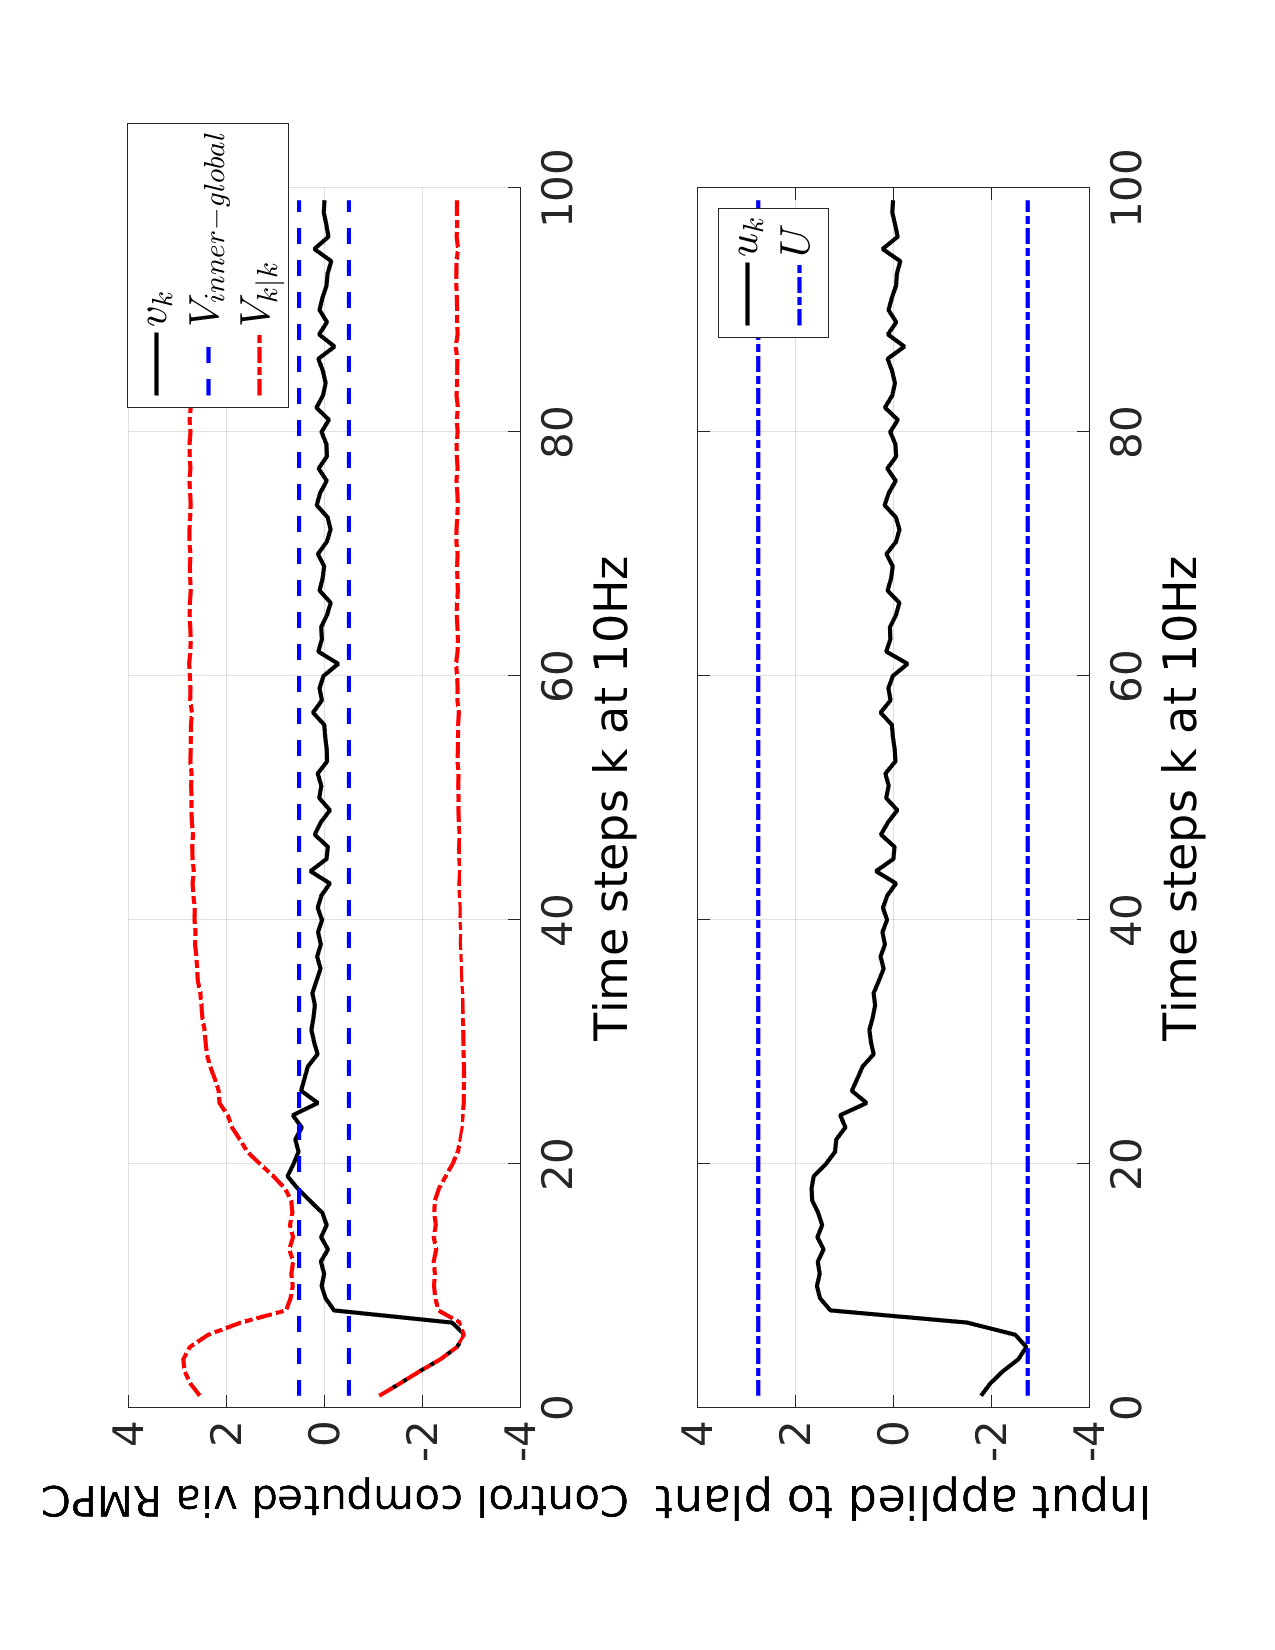
\includegraphics[angle=270,width=0.49\textwidth]{figs/u_and_v_toy.pdf}
	\caption{Inputs $v$ and $u$ and their bounds for the running example.}
	\label{fig:input toy}
\end{figure}

For the running example of Eq. \ref{eq:toy_dynamics}, we discretize the feedback linearized system at 10Hz and formulate the controller with a horizon of $N=15$ steps. 
The cost function has parameters $Q=I$ and $R=10^{-2}$.
The state trajectories (and estimates) for the nonlinear and linearized systems are shown in Fig. \ref{fig:AllStates_toy}.
Note that the states converges to the equilibrium 0 (and for the running example, $T$ preserves zero). 

\begin{figure}
	\centering	
	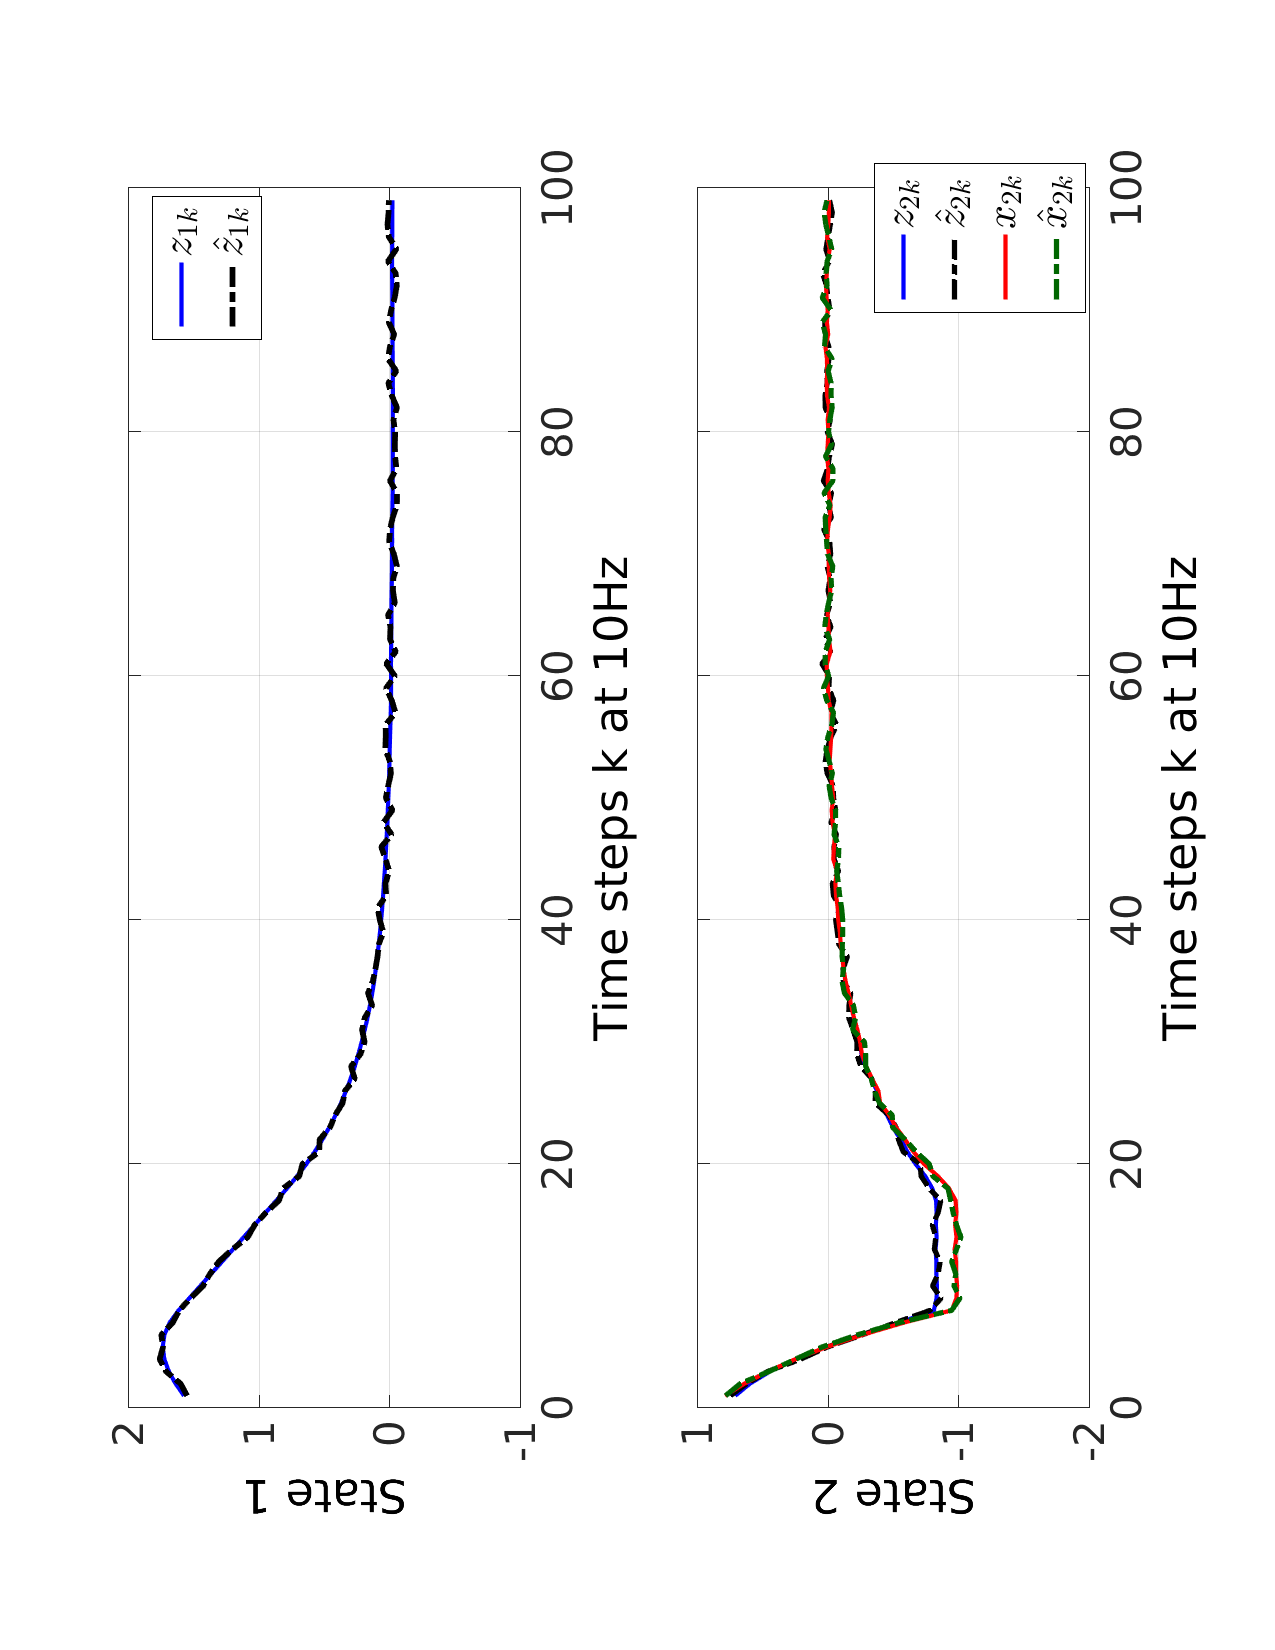
\includegraphics[angle=270,width=0.49\textwidth]{figs/AllStates_toy.pdf}
	\caption{The states and their estimates of the feedback linearized and non-linear running example. Recall that $z_1 = x_1$ therefore to reduce clutter, we only plot the first state only for the feedback linearized system.}
	\label{fig:AllStates_toy}
\end{figure}




%The input for the feedback linearized system is shown in Fig. ?? along with its upper and lower rectangular bounds computed online, denoted as $\oa{V}_{k|k}$ and $\ua{V}_{k|k}$ respectively, which make up the input constraint set at time $k$.
%Also shown is the global inner approximation $V_{inner-global}$ for the input $v$. 
%It is worth noting that the bounds computed online allow for much more control action than the conservative $V_{inner-global}$. 

The input $u$ is shown in Fig. \ref{fig:input toy}, and it can be noted that $u_k \in U$ for all $k$.

\subsection{Single link flexible joint manipulator}
\label{sec:manipulator}

\begin{figure}
	\includegraphics[scale=0.15]{figs/ManipArm.pdf}
	\caption{Flexible joint manipulator, figure from \cite{intech}.}
	\label{fig:manipulator fig}
\end{figure}

We consider the single link flexible manipulator system $S$, also used in \cite{intech}  shown in Fig. \ref{fig:manipulator fig}, whose dynamics are given by:
\begin{equation}
S: \begin{bmatrix} \dot{x}_1 \\ \dot{x}_2 \\ \dot{x}_3 \\ \dot{x}_4    \end{bmatrix} = \begin{bmatrix} x_2 \\ -\frac{mgl}{I}sin(x_1) - \frac{k}{I}(x_1-x_3)  \\ x_4 \\ \frac{k}{J}(x_1-x_3)  \end{bmatrix} + \begin{bmatrix} 0 \\ 0 \\ 0 \\ \frac{1}{J} \end{bmatrix}u
\end{equation}

This models a system where a motor, with an angular moment of inertia $J$,  is coupled to a uniform thin bar of mass $m=1/g$, length $l=1m$ and moment of inertia $I=1$, through a flexible torsional string with stiffness $k=1$. 
States $x_1$ and $x_2$ are the angles of the bar and motor shaft in radians, respectively, and $x_3, x_4$ are their respective rotational speeds in radians/sec.
The safe set is the box $X = [-\pi/4,\pi/4] \times [-\pi/4,\pi/4] \times [-\pi,\pi] \times [-\pi,\pi]$.
The input torque $u$ is bounded in $U = [\underline{u}, \overline{u}] = [-10 , 10 ]N\cdot m$. 
The estimation error $e = \hat{x} - x$ is bounded in $E = [-\pi /180, \pi /180]^4$.

The diffeomorphism $T$ is given by:
\begin{equation}
z = T(x) = \begin{bmatrix} x_1 \\ x_2 \\ -\frac{mgl}{I}sin(x_1) -\frac{k}{I}(x_1-x_3) \\ \frac{mgl}{I}x_2cos(x_1) - \frac{k}{I}(x_2-x_4)   \end{bmatrix}
\end{equation}

%For the linearization of Eq. ??, where $\hat{z}_k = z_k + M(x_k)e_k$, the matrix $M(x_k)$ is given by:
%\begin{equation}
%M(x_k) = \begin{bmatrix} 1&0&0&0 \\ 0&1&0&0 \\ -\frac{mgl}{I} cos(x_{1k}) -\frac{k}{I} &0 &\frac{k}{I} &0 \\ \frac{mgl}{I}x_{2k}sin(x_{1k}) & -\frac{mgl}{I} cos(x_{1k}) - \frac{k}{I} & 0 & \frac{k}{I}     \end{bmatrix}
%\end{equation}
The input to the feedback linearized system is given by $v=\beta u+ \alpha(x)$ where $\beta=\frac{k}{IJ} $ and 
\begin{subequations}
\label{eq:fblin_inp}
\begin{align}
\alpha(x)&=\frac{mgl}{I}x_2^2sin(x_1) + \frac{k^2}{IJ}(x_1-x_3) \nonumber \\
&- (\frac{mgl}{I}cos(x_1)-\frac{k}{I})(\frac{mgl}{I}sin(x_1)+\frac{k}{I}(x_1-x_3))
\end{align}
\end{subequations}

The feedback linearized system $S_{fl}$ has the dynamics:
$\dot{z_1} = z_2, \dot{z_2} = z_3, \dot{z_3} = z_4, \dot{z_4} = v$.
%\begin{subequations}
%\begin{align}
%\label{eq:fblin_manip}
%\dot{z_1} &= z_2 \\
%\dot{z_2} &= z_3 \\
%\dot{z_3} &= z_4 \\
%\dot{z_4} &= v
%\end{align}
%\end{subequations}


%\begin{figure}
%	\includegraphics[angle=270,width=0.49\textwidth]{figs/z_trajectory_new.pdf}
%	\caption{Evolution of $z_1$ and $z_2$, shown by the solid black line, inside the set Z (in red). The green sets are the reach sets $\oa{Z}_{k+i|k},\forall i=1,\dotsc,N, \forall k$. The light blue set is the one step ahead reach set $\oa{Z}_{k+1|k},\forall k$.}
%	\label{fig:z_new_toy}
%\end{figure}

A global inner approximation of the $v$ input set is computed, via interval arithmetic, as $V_{inner-global} = [max_{x\in X}\alpha(x) + \beta \underline{u}, min_{x\in X}\alpha(x) + \beta \overline{u}]$. 
Similarly, the inner approximations $\ua{V}_{k+j|k}$ are computed online by interval arithmetic as $\ua{V}_{k+j|k} = [max_{x\in \oa{X}_{k+j|k}} \alpha(x) + \beta \underline{u},  min_{x\in \oa{X}_{k+j|k}}\alpha(x) + \beta \overline{u}]$. 
Using the procedure of Sec. \ref{sec:transforming x to z} the set of states for $S_{fl}$ is given by $Z = [-0.5121, 0.5121]^2 \times [-2.5347, 2.5347] \times [-2.5603, 2.5603]$. Also $X_0 = [-0.4655,0.4655]^2 \times [-2.7598,2.7598] \times [-2.793,2.793]$. Comparing it to the set $X$, it shows that we can stabilize the system starting from initial states in a significantly large region in $X$.

We applied our controller to the above system with a discretization rate of 10Hz and MPC horizon $N=10$.
Fig.\ref{fig:AllStates_manip} show the states of the feedback linearized system $S_{fl}$. 
They converge to the origin in the presence of estimation error, while respecting all constraints.
Fig. \ref{fig:AllStates_manip} also shows $x_3$ and $x_4$: they also converge to zero (and remember $x_1 = z_1$ and $x_2 = z_2$).

\begin{figure}
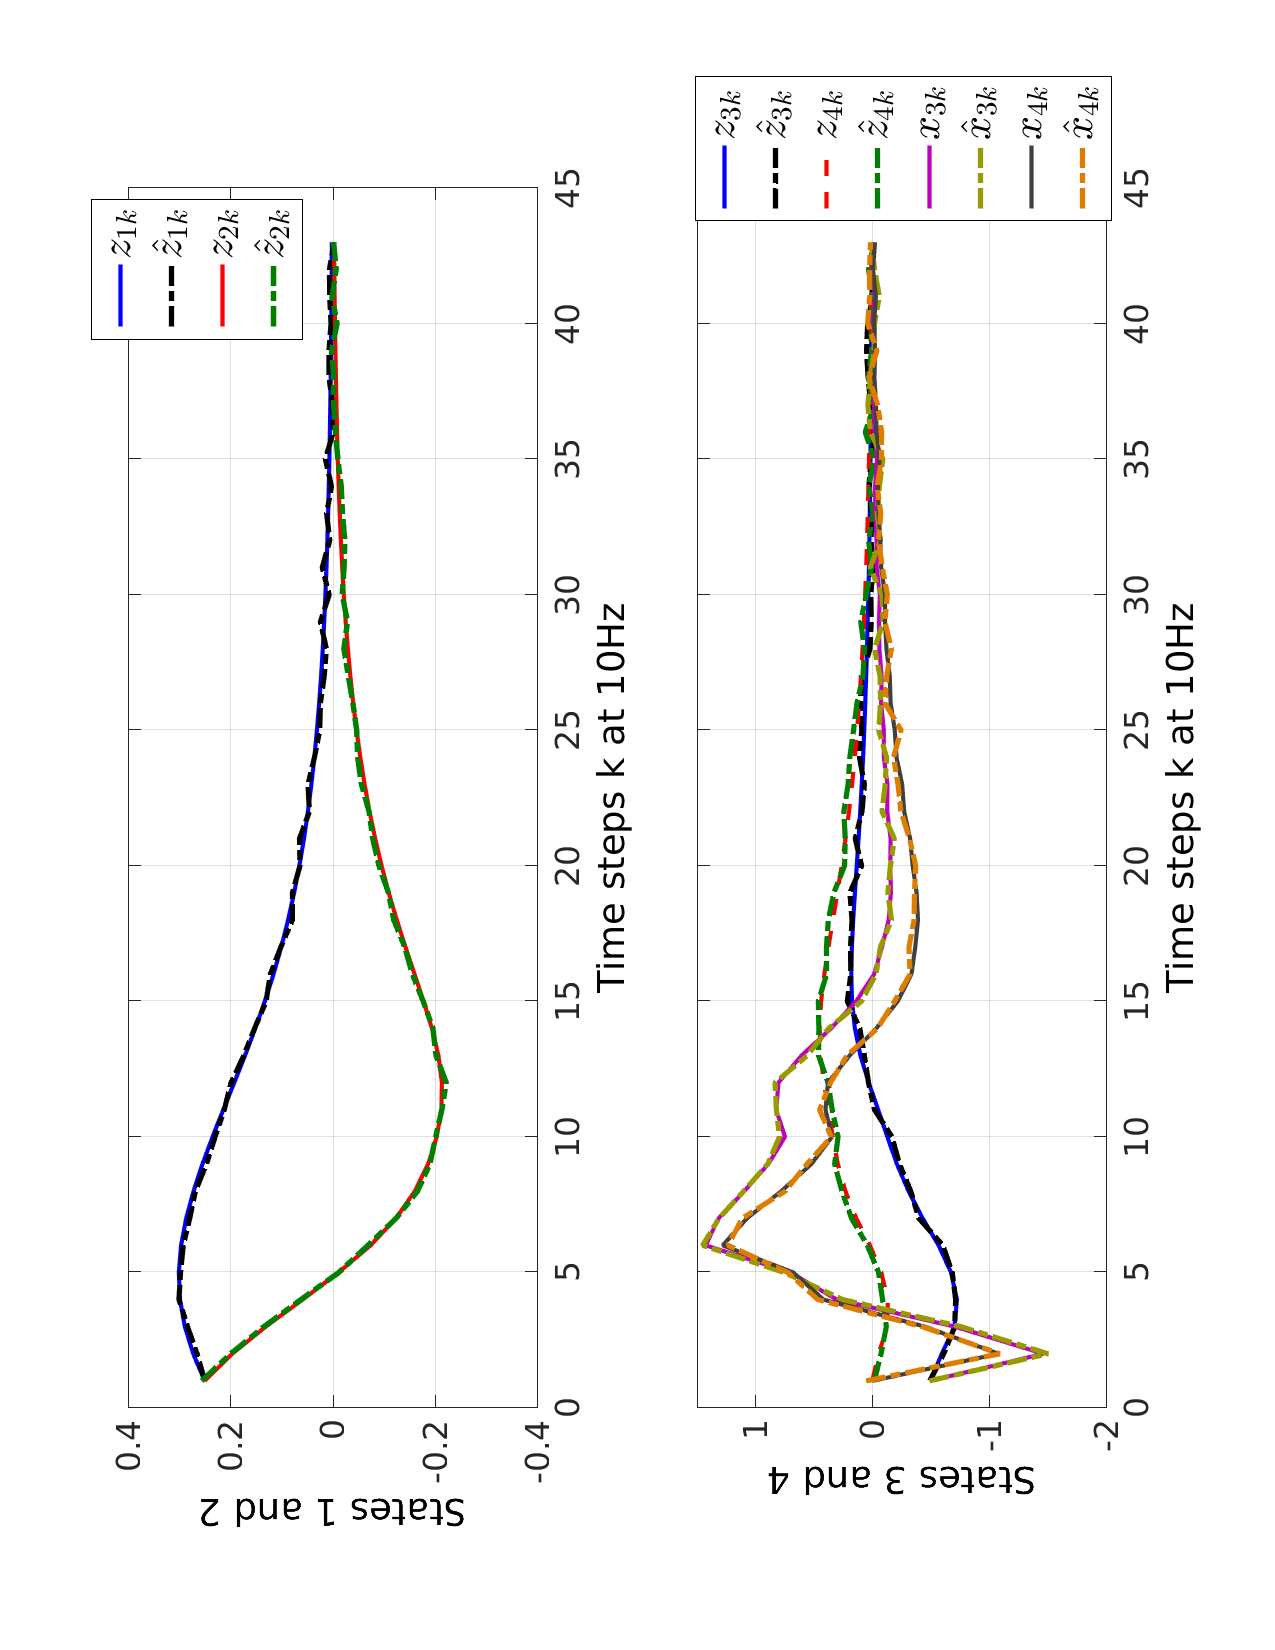
\includegraphics[angle=270,width=0.49\textwidth]{figs/AllStates_manip.pdf}
\caption{The states and their estimates of the feedback linearized and non-linear manipulator. Recall that $z_1 = x_1$ and $z_2=x_2$, therefore to reduce clutter, we only plot first two states only for the feedback linearized system.}
\label{fig:AllStates_manip}
\end{figure}

%\begin{figure}
%\includegraphics[width=0.49\textwidth]{figs/z_1n2_manip.pdf}
%\caption{$z_1$ and $z_2$ and their estimates $\hat{z_1}, \, \hat{z_2}$ vs time. Recall $z_1=x_1, z_2 = x_2$.}
%\label{fig:z_12}
%\end{figure}


%\begin{figure}
%\includegraphics[width=0.49\textwidth]{figs/z_1n2_manip.pdf}
%\caption{$z_1$ and $z_2$ and their estimates $\hat{z_1}, \, \hat{z_2}$ vs time. Recall $z_1=x_1, z_2 = x_2$.}
%\label{fig:z_12}
%\end{figure}

%\begin{figure}
%\includegraphics[width=0.49\textwidth]{figs/z_3n4_manip.pdf}
%\caption{$z_3$ and $z_4$ and their estimates $\hat{z_3}, \, \hat{z_4}$ vs time. }
%\label{fig:z_34}
%\end{figure}

Fig. \ref{fig:v_and_limits} shows the input $v$ to $S_{fl}$ $v$ along with the global inner approximation $V_{inner-global}$ and the $x$-dependent inner approximations $\ua{V}_{k+k|k}$ computed online.
Note that the bounds computed online allow for significantly more control action compared to the conservative global inner approximation. 
Finally, Fig. \ref{fig:v_and_limits} also shows the input $u$ applied to the non-linear system (and its bounds), which robustly respects its constraints $u \in U$.

%\begin{figure}
%\includegraphics[width=0.49\textwidth]{figs/x_3n4_manip.pdf}
%\caption{$x_3$ and $x_4$ and their estimates $\hat{x_3}, \, \hat{x_4}$ vs time. }
%\label{fig:x_34}
%\end{figure}


\begin{figure}
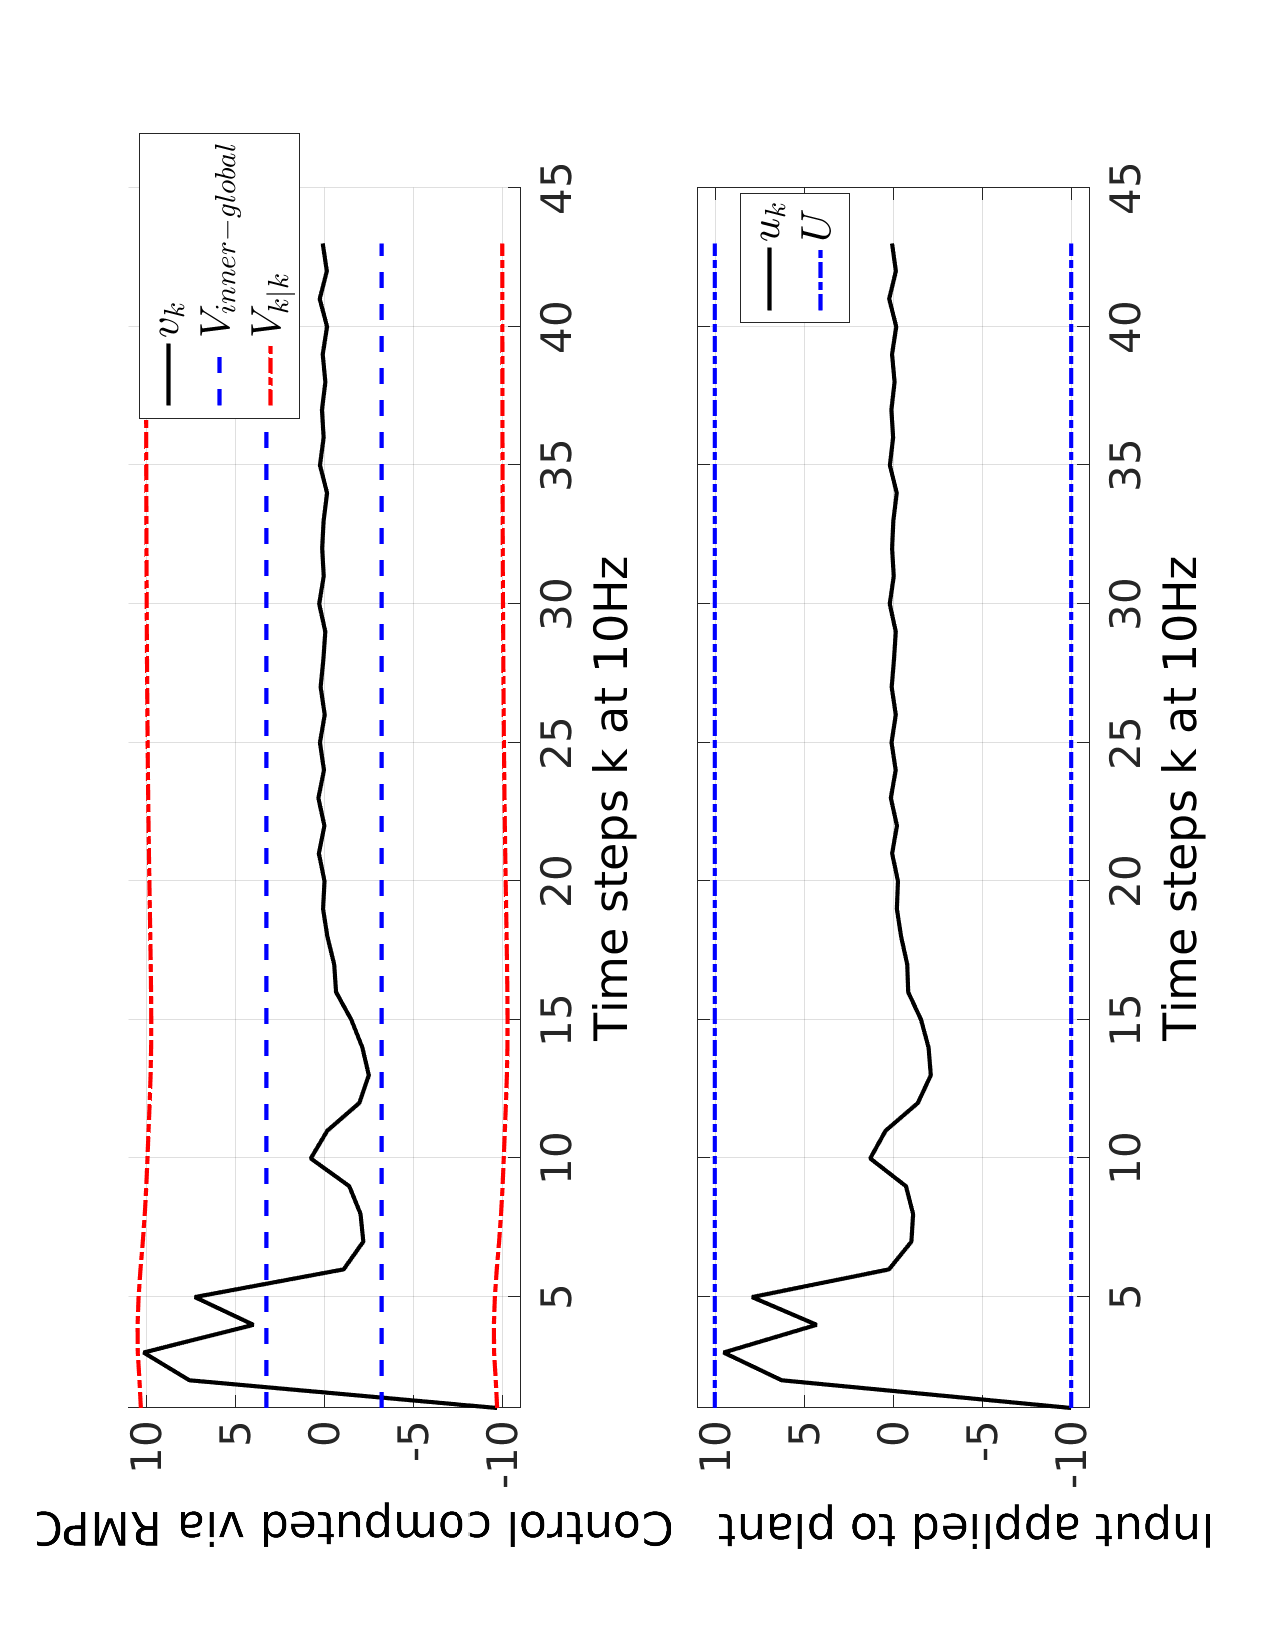
\includegraphics[angle=270,width=0.49\textwidth]{figs/u_and_v_manip.pdf}
\caption{Inputs $v$ and $u$ and their bounds for the manipulator example .}
\label{fig:v_and_limits}
\end{figure}



%\begin{figure}
%\includegraphics[width=0.49\textwidth]{figs/v_and_limits_manip.pdf}
%\caption{Input to the feedback linearized system and its bounds.}
%\label{fig:v_and_limits}
%\end{figure}

%\begin{figure}
%\includegraphics[width=0.49\textwidth]{figs/u_and_limits_manip.pdf}
%\caption{Input to the non-linear system and its upper and lower limits.}
%\label{fig:u_and_limits}
%\end{figure}



\section{Conclusion}
\label{conclusion}

In this paper we presented a contract-based methodology for co-design of estimation and control for autonomous systems. 
The basic idea is that the control algorithm requests a time and estimation error $\de$ contract that the perception-and-estimation algorithm realizes. The control algorithm we designed aims to set time varying contracts to maximise a performance function while guaranteeing feasibility constraints and stability under the time varying execution time and estimation error from the estimator. We also illustrate how the contract based perception-and-estimation algorithm is designed offline and used at run-time to best meet the $\de$ contracts set for it. Through a case study on a flying hex-rotor, we showed the applicability of our scheme to real-time closed loop system. The experimental results show the good performance of our scheme and how it outperforms regular Model Predictive Control which does not leverage co-design. A key result showed how our closed loop solution is more energy efficient than MPC while achieving better tracking performance. A focus of ongoing research is to overcome the necessity of the contracts always being met by the estimator in order of us to have strong mathematical guarantees for the control performance. Another focus is on an automated tool chain to profile perception algorithms commonly used in autonomous systems.
%\section*{Appendix}

\subsection{Constraints of successive MPC problems}
\label{sec:inclusions statement}
We are now ready to state and prove a key lemma regarding the evolution of the state, error and input sets between MPC optimization problems. 
This lemma will be key to proving recursive feasibility of the MPC controller, since it allows us to show that the constraint sets of one problem, at time $k$, are appropriate supersets of the constraint sets of the next problem, at time $k+1$. 

\begin{lemma}
	\label{lem:set inclusions}
	Let $\oa{X}_{k+j|k}$ be the $j$-step outer-approximate reach set computed at time $k$ by a reachability tool as described in Sec. \ref{sec:x reach}.
	
	Let $\What_{k+j|k}$ be the set defined in \eqref{eq:What}.
	
	Let $\tE_{k+j|k}$ be the error set computed using \eqref{eq:H}, \eqref{eq:tildeE} by substituting $E \leftarrow \tE_{k|k}$.
	
	Let $\ua{V}_{k+j|k} = \ua{V}(\oa{X}_{k+j|k})$ and $\oa{V}_{k+j|k} = \oa{V}(\oa{X}_{k+j|k})$ 

Then the following hold for all $k \geq 0, ,j \geq 1$:
\begin{enumerate}
	\item $\oa{X}_{k+1+j|k+1} \subseteq \oa{X}_{k+j+1|k}$
	\label{set:X}
	\item $\tE_{k+1+j|k+1} \subseteq \tE_{k+j+1|k}$
	\label{set:tE}
	\item $\What_{k+1+j|k+1} \subseteq \What_{k+j+1|k}$
	\label{set:What}
	\item $\oa{V}_{k+1+j|k+1} \subseteq \oa{V}_{k+j+1|k}$
	\label{set:oaV}
	\item $\ua{V}_{k+1+j|k+1} \supseteq \ua{V}_{k+j+1|k}$ (note the change in inclusion direction)
	\label{set:uaV}		
\end{enumerate} 
\end{lemma} 

\begin{proof}
	
\ref{set:X}) 
Fix an arbitrary $k$. We prove this by induction on $j \geq 1$.

\underline{Base case: $j=1$}. By construction, $\hx_{k+1} \in \RT{\Xset{k}{k}} \oplus E$.
Therefore at time $k+1$, when setting up the problem $\mathbb{P}_{k+1}(\hat{z}_{k+1})$, the algorithm will first compute
$\Xset{k+1}{k+1} = \hx_{k+1} \oplus (-E)  \subset \RT{\Xset{k}{k}} \oplus E \oplus (-E) = \oaXset{k+1}{k}$.
Also 
$\oaXset{k+2}{k+1} = \RT{\Xset{k+1}{k+1}} \oplus E \oplus(-E) \subset  \RT{\oaXset{k+1}{k}} \oplus E \oplus(-E) = \oaXset{k+2}{k}$.

\underline{Induction step: $j > 1$}.
By definition, $\oaXset{k+1+j}{k+1} = \RT{\oaXset{k+1+j-1}{k+1}} \oplus E \oplus (-E) \subset  \RT{\oaXset{k+j}{k}} \oplus E \oplus (-E)$ (by the induction hypothesis). This last set equals $\oaXset{k+j+1}{k}$ by definition.

\ref{set:tE}) 	By \ref{set:X}) 
 we have that 
 $ \min_{x \in \oa{X}_{k+j+1|k}, e \in E} M_{i\ell}(x)e(\ell) \leq \min_{x \in \oa{X}_{k+1+j|k+1}, e \in E} M_{i\ell}(x)e(\ell)$ and that 
 $\max_{x \in \oa{X}_{k+j+1|k}, e \in E} M_{i\ell}(x)e(\ell) \leq \max_{x \in \oa{X}_{k+1+j|k+1}, e \in E} M_{i\ell}(x)e(\ell)$
 which yields the desired result.
 
 \ref{set:What}) This is immediate from the definition \eqref{eq:What} and \ref{set:tE}).
 
 \ref{set:oaV}) and \ref{set:uaV}) These are immediate from \eqref{eq:V inclusions}.
 
	\end{proof}


\subsection{Proof of Theorem \ref{th:robust_feas}}
\label{sec:proof of thm 1}
We will prove the Theorem by recursion by showing that if at time step $k$, the problem $\mathbb{P}_{k}(\hat{z}_k)$ is feasible and the feasible control input $v_k = v^{*}_{k|k}$ is applied, then $v_k$ is admissible (meets the system constraints) and at time $k+1$, $z_{k+1}$ is inside $Z$ and also $\mathbb{P}_{k+1}(\hat{z}_{k+1})$ is feasible for all disturbances. By recursion then, if we have feasibility at step $k=k_0$, we have robust constraint satisfaction and feasibility at time step $k_0+1$ and so on for all $k>k_0$. 

To begin, let $\mathbb{P}_{k}(\hat{z}_k)$ be feasible, then it has a feasible solution $(\lbrace z^{*}_{k+j|k}\rbrace_{j=0}^{N+1}, \, \lbrace v^{*}_{k+j|k}\rbrace_{j=0}^{N} )$ that satisfies all the constraints of the Robust MPC. 
Now let's construct a feasible candidate solution for $\mathbb{P}_{k+1}(\hat{z}_{k+1})$ at the next time step by shifting the above solution one-step forward. 
Consider the candidate solution:

\begin{subequations}
\begin{align}
\label{eq:candidate}
\nz_{k+j+1|k+1} &= z^{*}_{k+j+1|k} + L_j\hat{w}_{k+1}, \, \forall j \in [0:N]\\
\nz_{k+N+2|k+1}&= A\nz_{k+N+1|k+1} + B\bar{v}_{k+N+1|k+1} \\
\bar{v}_{k+j+1|k+1}&=v^{*}_{k+j+1|k} + KL_j\hat{w}_{k+1}, \, \forall j \in [0:N-1]\\
\bar{v}_{k+N+1|k+1}&=K\nz_{k+N+1|k+1} 
\end{align}
\end{subequations}

First we will show that the input and state constraints are satisfied by $v_k$ and $\nz_{k+1}$, then prove feasibility of the above candidate solution for $\mathbb{P}_{k+1}(\hat{z}_{k+1})$.

\textit{Validity of input and next state:}
The next state is:
\begin{eqnarray}
\label{eq:z_next}
z_{k+1} &= &Az_k + Bv_k + w_k \nonumber
\\
&=& A(\hat{z}_k-\tilde{e}_k)+Bv^{*}_{k|k}+w_k \nonumber \\
 &=& A\hat{z}_k+Bv^{*}_{k|k}-\tilde{e}_{k+1}+(w_k+\tilde{e}_{k+1}-A\tilde{e}_k) \nonumber \\
  &=& Az^{*}_{k|k} +Bv^{*}_{k|k}-\tilde{e}_{k+1}+  \hw_{k+1} \nonumber\\
  & \;& \quad (\Pk{k} \text{ initialization}) \nonumber \\
&= &z^{*}_{k+1|k} - \tilde{e}_{k+1} + \hat{w}_{k+1} 
\end{eqnarray}

By feasibility of the solution at time $k$,
\begin{equation*}
z^{*}_{k+1|k} \in\nomZset{k+1}{k} = Z \ominus (-\tilde{E}_{k+1|k}) \ominus L_0\What_{k+1|k}
\end{equation*}

Therefore, $z_{k+1} \in Z$ and so $x_{k+1} \in X$.
%By definition, $\tilde{e}_{k+1} \in \tilde{E}_{k+1|k}$ and $\hat{w}_{k+1} \in  \What_{k+1|k}$. Using this fact, definition of Pontraygin difference and Eq. \ref{eq:z_next} (also remember, $L_0 = \mathbb{I}$), we have that:

Moreover, by the feasibility of $v^{*}_{k|k}$ for $\mathbb{P}_{k}(\hat{z}_k)$ and by the definition of $\underline{V}_{k|k}$,
$v_k = v^{*}_{k|k} \in \underline{V}_{k|k}$, which implies that $u_k \in U$.

Hence, if $\mathbb{P}_{k}(\hat{z}_k)$ is feasible, then the applied input at time step $k$ and the resulting next state $z_{k+1}$ (and hence $x_{k+1}$) are admissible under all possible disturbances. 
The next part of the proof will focus on showing that the candidate solution of Eq. \eqref{eq:candidate} is indeed feasible for $\Pk{k+1}$ by proving that it meets all the constraints.

\textit{Initial Condition:} Recall from \eqref{eq:dynamics_estimate} that $\hat{z}_{k+1} = A\hat{z}_k + Bv_k + \hat{w}_{k+1}$.
Also by the construction of the candidate solution,
\begin{subequations}
\begin{align}
\nz_{k+1|k+1} &= z^{*}_{k+1|k} + L_0 \hat{w}_{k+1} \nonumber \\
&= Az^{*}_{k|k} + Bv^{*}_{k|k} + \hat{w}_{k+1}
\end{align}
\end{subequations}

Since $z^{*}_{k|k}=\hat{z}_k$ and $v^{*}_{k|k} = v_k$, by the two equations above, we have
\begin{equation}
\nz_{k+1|k+1} = \hat{z}_{k+1}
\end{equation}

Hence, the candidate solution does indeed satisfy the initial condition for $\Pk{k+1}$.
Next we show that the candidate solution satisfies the nominal dynamics:

\textit{ Nominal Dynamics:} For $0\leq j<N$,we have:
\begin{eqnarray*}
&& \nz_{k+j+2|k+1} 
\\
&& = z^{*}_{k+j+2|k} + L_{j+1}\hat{w}_{k+1} \\
&& = Az^{*}_{k+j+1}+Bv^{*}_{k+j+1|k} + L_{j+1}\hat{w}_{k+1} \\
&& \text{By the construction of the candidate solution} \nonumber \\
&& = A(\nz_{k+j+1|k+1}-L_j\hat{w}_{k+1}) + B(\bar{v}_{k+j+1|k+1} - KL_j \hat{w}_{k+1}) \nonumber \\
&& \;\; + L_{j+1}\hat{w}_{k+1} \\
&& = A\nz_{k+j+1|k+1} + B\bar{v}_{k+j+1|k+1} -(A+BK)L_j\hat{w}_{k+1} \nonumber \\
&& \;\; + L_{j+1}\hat{w}_{k+1} \\
&& = A\nz_{k+j+1|k+1} + B\bar{v}_{k+j+1|k+1} - L_{j+1}\hat{w}_{k+1} + L_{j+1}\hat{w}_{k+1} \\
&& = A\nz_{k+j+1|k+1} + B\bar{v}_{k+j+1|k+1}
\end{eqnarray*}

For $j=N$, by construction $\nz_{k+N+2|k+1} = A\nz_{k+N+1|k+1} + B\bar{v}_{k+N+1|k+1}$. Hence, the candidate solution does indeed satisfy the nominal dynamics.

\textit{State Constraints:} To show feasibility of the candidate solution w.r.t the state constraints, we need to show that $\nz_{(k+1)+j|k+1}\in \nomZset{k+1+j}{k+1}\, \forall j=0,\dotsc,N$. Re-writing Eq.\ref{eq:Set_constraints} for $\mathbb{P}_{k}(\hat{z}_k)$ for $j=0,\dotsc,N-1$, we have:

\begin{subequations}
\label{eq:redef_Zj}
\begin{align}
& \nomZset{k+j+1}{k} \nonumber
\\
\; \; &= Z \ominus_{i=0}^{j}L_i\What_{k+j+1-i|k} \ominus (-\tilde{E}_{k+j+1|k}) \nonumber \\
 &= Z \ominus L_j \What_{k+1|k} \ominus_{i=1}^{j}L_i\What_{k+j+1-i|k} \ominus (-\tilde{E}_{k+j+1|k}) \nonumber\\
 &= Z \ominus L_j \What_{k+1|k} \ominus_{i=0}^{j-1}L_i\What_{k+j-i|k} \ominus (-\tilde{E}_{k+j+1|k}) \nonumber
\end{align}
\end{subequations}


Also, let us write the state constraints for all $j=0,\dotsc,N$ for the problem at time $k+1$, i.e. for $\mathbb{P}_{k+1}(\hat{z}_{k+1})$:
\begin{equation*}
\label{eq:redef_Zjp1}
\nomZset{(k+1)+j}{k+1} = Z \ominus_{i=0}^{j-1}L_i\What_{k+j-i|k+1} \ominus (-\tilde{E}_{k+1+j|k+1}) \\
\end{equation*}

Remember, by construction of the candidate, we have $\nz_{k+j+1|k+1} = z^{*}_{k+j+1|k} + L_j\hat{w}_{k+1}$.
Also by feasibility of the algorithm at time $k$, we have $z^{*}_{k+j+1|k}\in \nomZset{k+j+1}{k}$, and by definition, $L_j\hat{w}_{k+1} \in L_j\What_{k+1|k}$. 
Therefore by Eq. \eqref{eq:redef_Zj}, we have $\forall j=0,\dotsc,N-1$,
\begin{equation}
\nz_{(k+1)+j|k+1} \in Z \ominus_{i=0}^{j-1}L_i\What_{k+j-i|k} \ominus (-\tilde{E}_{k+j+1|k}) \\
\end{equation}
Using points 2) and 3) from Lemma \ref{lem:set inclusions},
\begin{eqnarray*}
&&Z \ominus_{i=0}^{j-1}L_i\What_{k+j-i|k} \ominus (-\tilde{E}_{k+j+1|k})
\nonumber
\\
&&\;\;  \subseteq Z \ominus_{i=0}^{j-1}L_i\What_{k+j-i|k+1}  \ominus (-\tilde{E}_{k+j+1|k+1}) 
\end{eqnarray*}
And using Eq. \eqref{eq:redef_Zjp1}, this implies for all $j=0,\dotsc,N-1$
\[\nz_{(k+1)+j|k+1} \in \nomZset{k+1+j}{k+1}\]

Now for $j=N$, $\nz_{k+N+1|k+1} = z^{*}_{k+N+1|k} + L_N\hat{w}_{k+1}$. 
From the terminal constraint we have $[z^{*}_{k+N+1|k}\, v^{*}_{k+N|k}] \in P_f = C_p \ominus \hat{L}_N\hat{F}\What_{max}$. Since $w_{k+1} \in \What_{max}$, and by the construction of the candidate solution

\begin{equation}
\label{eq:CandidateInC}
[\nz_{k+N+1|k+1}\, \bar{v}_{k+N|k+1}] \in C_p
\end{equation}

Remember, by definition of the invariant set, $C_p \in P_N(\tilde{E}_{max},\tilde{E}_{max})$, and since by definition of $\tilde{E}_{max}$ and Eq. \ref{eq:Set_constraints}, we have $P_N(\tilde{E}_{max},\tilde{E}_{max}) \subseteq \nomZset{k+1+N}{k+1} \times V_{k+1+N|k+1}$, or $C_p \in  \nomZset{k+1+N}{k+1} \times {V}_{k+1+N|k+1}$. This implies that $\nz_{k+N+1|k+1} \in \nomZset{k+1+N}{k+1}$ and additionally, $v_{k+N|k+1} \in {V}_{k+1+N|k+1}$.
Therefore, the set constraints are met by candidate solution $\forall j=0,\dotsc,N$. 

\textit{Input Constraints:} For the inputs, we show that the candidate solution, $\bar{v}_{k+j+1|k+1}, j=0,\ldots,N-2$, satisfies the input constraints for $\mathbb{P}_{k+1}(\hat{z}_{k+1}) $ by using a similar argument as that used for the state constraints. 
Let us re-write the input constraints for $\mathbb{P}_{k}(\hat{z}_{k})$ for $j=0,\dotsc,N-2$,

\begin{subequations}
\label{eq:V_redef}
\begin{align}
V_{k+j+1|k}&=\underline{V}_{k+j+1|k} \ominus_{i=0}^{j} KL_i\What_{k+j+1-i|k} \\
&=\underline{V}_{k+j+1|k} \ominus KL_jW_{k+1|k} \ominus_{i=1}^{j} KL_i\What_{k+j+1-i|k} \\
&=\underline{V}_{k+j+1|k} \ominus KL_jW_{k+1|k} \ominus_{i=0}^{j-1} KL_i\What_{k+j-i|k}
\end{align}
\end{subequations}

Let us also re-write the input constraints for $\mathbb{P}_{k+1}(\hat{z}_{k+1})$ for $j=0,\dotsc,N-1$,
\begin{equation}
\label{eq:Vjkp1}
V_{k+1+j|k+1}=\underline{V}_{k+j+1|k+1} \ominus_{i=0}^{j-1} KL_i\What_{k+j-i|k+1}
\end{equation}

By construction of the candidate, we have $\bar{v}_{k+1+j|k+1}=v^{*}_{k+j+1|k}+KL_j\hat{w}_{k+1}$. Also by feasibility of the algorithm at time $k$, we have $v^{*}_{k+j+1|k} \in V_{k+j+1|k}$, and by definition, $L_j\hat{w}_{k+1} \in L_j\What_{k+1|k}$. Therefore by definition of the Pontraygin difference and Eq. \ref{eq:V_redef}, we have $\forall j=1,\dotsc,N-1$,
\begin{subequations}
\begin{align}
&\bar{v}_{(k+1)+j|k+1} \in \underline{V}_{k+j+1|k} \ominus_{i=0}^{j-1}L_i\What_{k+j-1|k} \\
&\text{Using points 3) and 4) from Lemma \ref{lem:one}} \nonumber \\
&\underline{V}_{k+j+1|k} \ominus_{i=0}^{j-1}L_i\What_{k+j-1|k} \subseteq \nonumber \\
& \qquad \underline{V}_{k+j+1|k+1} \ominus_{i=0}^{j-1}L_i\What_{k+j-1|k+1} \\
&\text{And using Eq. \ref{eq:Vjkp1}, this implies} \nonumber \\
&\bar{v}_{(k+1)+j|k+1} \in V_{k+1+j|k+1}
\end{align}
\end{subequations}

Note,  for $j=N-1$, we have already shown in the proof for the state constraints that by definition of the invariant set $C$, $v_{k+N|k+1} \in {V}_{k+1+N-1|k+1}$ by respecting an even tighter constraint.
For the last input for $j=N$, we have $\bar{v}_{k+1+N|k+1}=K\nz_{k+N+1|k}$, we show that it is inside the (joint) terminal constraint $P_f$, and hence is feasible.

\textit{Terminal Constraints:} Finally, we need to show that $[\nz_{k+N+2} \, \bar{v}_{k+N+1}]' \in P_f$. This can be shown using the construction of the terminal set and the candidate solution. From Equation \ref{eq:candidate}, we have:
\begin{subequations}
\begin{align}
\nz_{k+N+2|k+1}&=A\nz_{k+N+1|k+1} + B\bar{v}_{k+N+1|k} \\
\bar{v}_{k+N+1|k+1}&=K\nz_{k+N+1|k+1}
\end{align}
\end{subequations}

Concatenate these two into $p_{k+N+2|k+1} = [\nz_{k+N+2|k+1}\, \bar{v}_{k+N+1|k+1}]'$. Also $p_{k+N+1|k+1} = [\nz_{k+N+1} \,\bar{v}_{k+N}]^T$ was in $C_p$ as shown previously (Eq. \ref{eq:CandidateInC}). 
Therefore, by definition of the invariant set $C_p$ (Equation \ref{eq:C_def}), we have that $p_{k+N+2|k+1} + \hat{L}_N \hat{F} w_{k+1|k}\in C_p$ for all $w_{k+1|k}\in \What_{k+1|k} \subseteq \What_{max}$. 
Therefore $p_{k+N+2|k+1} \in C_p \ominus \hat{L}_N\hat{F}\What_{max} = P_f$. 
Therefore the terminal constraint is also met.

With this, we have the proof for Theorem 1 as we have shown that feasible solution at time step $k$ for $\mathbb{P}_{k}(\hat{z}_{k}) $ implies that the applied input $v_k$ is feasible, the next state $z_{k+1} \in Z$ and the problem $\mathbb{P}_{k+1}(\hat{z}_{k+1}) $ is feasible at time $k+1$, and hence  $\mathbb{P}_{k+2}(\hat{z}_{k+2}) $ is feasible for time step $k+2$ and so on. $\blacksquare$


% =================================
\subsection{Proof of Thm. \ref{thm:stability}}
	Let $T$ be the diffeomorphism mapping $x$ to $z$ from feedback linearization, and set $z_e = T(x_e)$. 
	Since $x_e$ is an equilibrium point, $z_e=0$.
	%By a change of variables $z' = z - T(x_e)$, stabilizing the linear dynamics (with state $z'$) to 0 implies stabilizing the nonlinear dynamics to $x_e$.
	Recall that $Q$ and $Q_f$ of  \eqref{eq:nom mpc} are positive semi-definite and that $R$ is positive definite,  so that the optimal cost $J^*(\nz_{k})$ is a positive definite function of $\nz_{k}$, and that the terminal weight in \eqref{eq:nom mpc} is equivalent to the infinite horizon cost (by our choice of $Q_f$). 
	Finally Thm.  \ref{th:robust_feas} guarantees that the tail of the input sequence computed at $k$ is admissible at time $k+1$. 
	Therefore it is a standard result that the optimal cost $J^{*}({\nz}_{k})$ is non-increasing in $k$ and that $0$ is a stable equilibrium for the closed-loop linear system (e.g., see \cite{CannonK15MPC} ). 
	Moreover, the terminal set $P_f$ is a robust invariant set of the $z$ dynamics containing 0 (see Section \ref{sec:Constraints}).
	Therefore Algorithm \ref{alg:RMPC} stabilizes the nominal state $\nz$ to $P_f$ from anywhere in $Z_0$, and the true (linearized) state $z$ to an invariant set $Z_{inv}$ around $0$, and the nonlinear state $x$ to the invariant set $X_{inv} = T^{-1}(Z_{inv})$.
	Therefore Algorithm \ref{alg:RMPC} drives $x$ to $X_{inv}$ from anywhere in $X_0 \subset \iT(Z)$.
	
% ====================================
\subsection{Transforming between $x$-space and $z$-space}
\label{sec:transforming x to z}
Since we control the system in $z$-space, we need to compute a set $Z \subset \Re^{\dimZ}$ s.t. $z \in Z \implies x = \iT(z) \in X$, i.e. $Z \subset T(X)$.
Thus keeping the state $z$ of the linearized dynamics in $Z$ implies the nonlinear system's state $x$ remains in $X$.
Moreover, to check feasibility at time 0 of the MPC optimization, and for stability of the nonlinear dynamics, we need a subset $X_0 \subset X$ s.t. $x \in X_0 \implies z = T(x) \in Z$, i.e. $X_0 \subset \iT(Z)$.
Because $T$ can be an arbitrary diffeomorphism $Z$ and $X_0$ have to computed numerically.
\begin{enumerate}
	\item Let $Z_1 \subset \Re^{\dimZ}$ be the rectangle with bounds in the $i^{th}$ dimension $[ \min_{x \in X} T_i(x),  \max_{x \in X} T_i(x) ]$, $i=1,\ldots, \dimX$.
	This over-approximates $T(X)$. 
	Next we need to prune it so it under-approximates $T(X)$. 
	\item Define $z_{in} \defeq \min \{ \|z \|_0 \such z \in Z_1, \iT(z) \notin X\}$.
	$z_{in}$ is the smallest-norm inadmissible $z$ in $Z_1$.
	Thus all points in the $\ell_0$-ball of radius $\|z_{in}\|$,$B_z(0,\|z_{in}\|)$, are admissible, i.e. their pre-images via $\iT$ are in $X$.
	\item Let $R_z$ be the largest inscribed rectangle in $B_z(0,\|z_{in}\|)$.
	Now we need to get the $x$-set that maps to $R_z$  (or a subset of it).
	\item Let $X_1 \subset X$ be the rectangle with bounds in the $i^{th}$ dimension $[\min_{z \in R_{z}} \iT_i(z),  \max_{z \in R_{z}} \iT_i(z) ]$.
	Again, this is an over-approximation of $\iT(R_{z})$, so it needs to be pruned.
	\item Define $x_{in} = \inf \{\|x\|_0 \such x \in X_1, T(x) \notin R_{z}\}$.
	Then every point in the $\ell_0$-ball $B_x(0, \|x_{in}\|) \subset X$ maps via $T$ to $R_{z}$
\end{enumerate}
Therefore we choose $Z = R_z$ and $X_0$ to be the largest inscribed rectangle in $B_x(0,  \|x_{in}\|)$.

% ====================================
\subsection{Error sets}
For the running example, Fig. \ref{fig:err_bound_toy} shows the set $\tE_{max}$ and $\tilde{E}_{k+j|k}$ computed by Eqs. \eqref{eq:tildeE} and \eqref{eq:EtildeMax}. for an arbitrary  $\oa{X}_{k+j|k} =  [-\pi/4,0]\times[-0.9666,-0.6283]$. 
It also shows 1000 randomly generated values for $T(\hat{x})-x$ (for randomly generated $e \in E$ and $x \in \oa{X}_{k+j|k}$), and all fall inside $\tilde{E}_{k+j|k}$.

%computed over $\Xc= [-\pi/4,0]\times[-0.9666,-0.6283]$. 
%This shows that considering a reach set $\chi \subseteq X$ to compute the error bound results in less conservatism than using the worst case error bound. It also shows randomised realizations of the error for randomly selected $x \in \chi$ and $e \in E$, which %are all contained in the bounding set $\tilde{E}_{\chi}$.

\begin{figure}
	\includegraphics[angle=270,width=0.49\textwidth]{figs/Err_Bounds_toy.pdf}
	\caption{The error sets $\tilde{E}_{max}$ and $\tilde{E}$ computed over an arbitrary $\oa{X}_{k+j|k}$. Also shown are realizations of $\te \defeq T(\hx) - T(x)$ for randomly chosen $x \in \Xc$. Color in online version.}
	\label{fig:err_bound_toy}
\end{figure}

% ====================================
\subsection{Experiments with the Running example}

\begin{figure}
	\centering	
	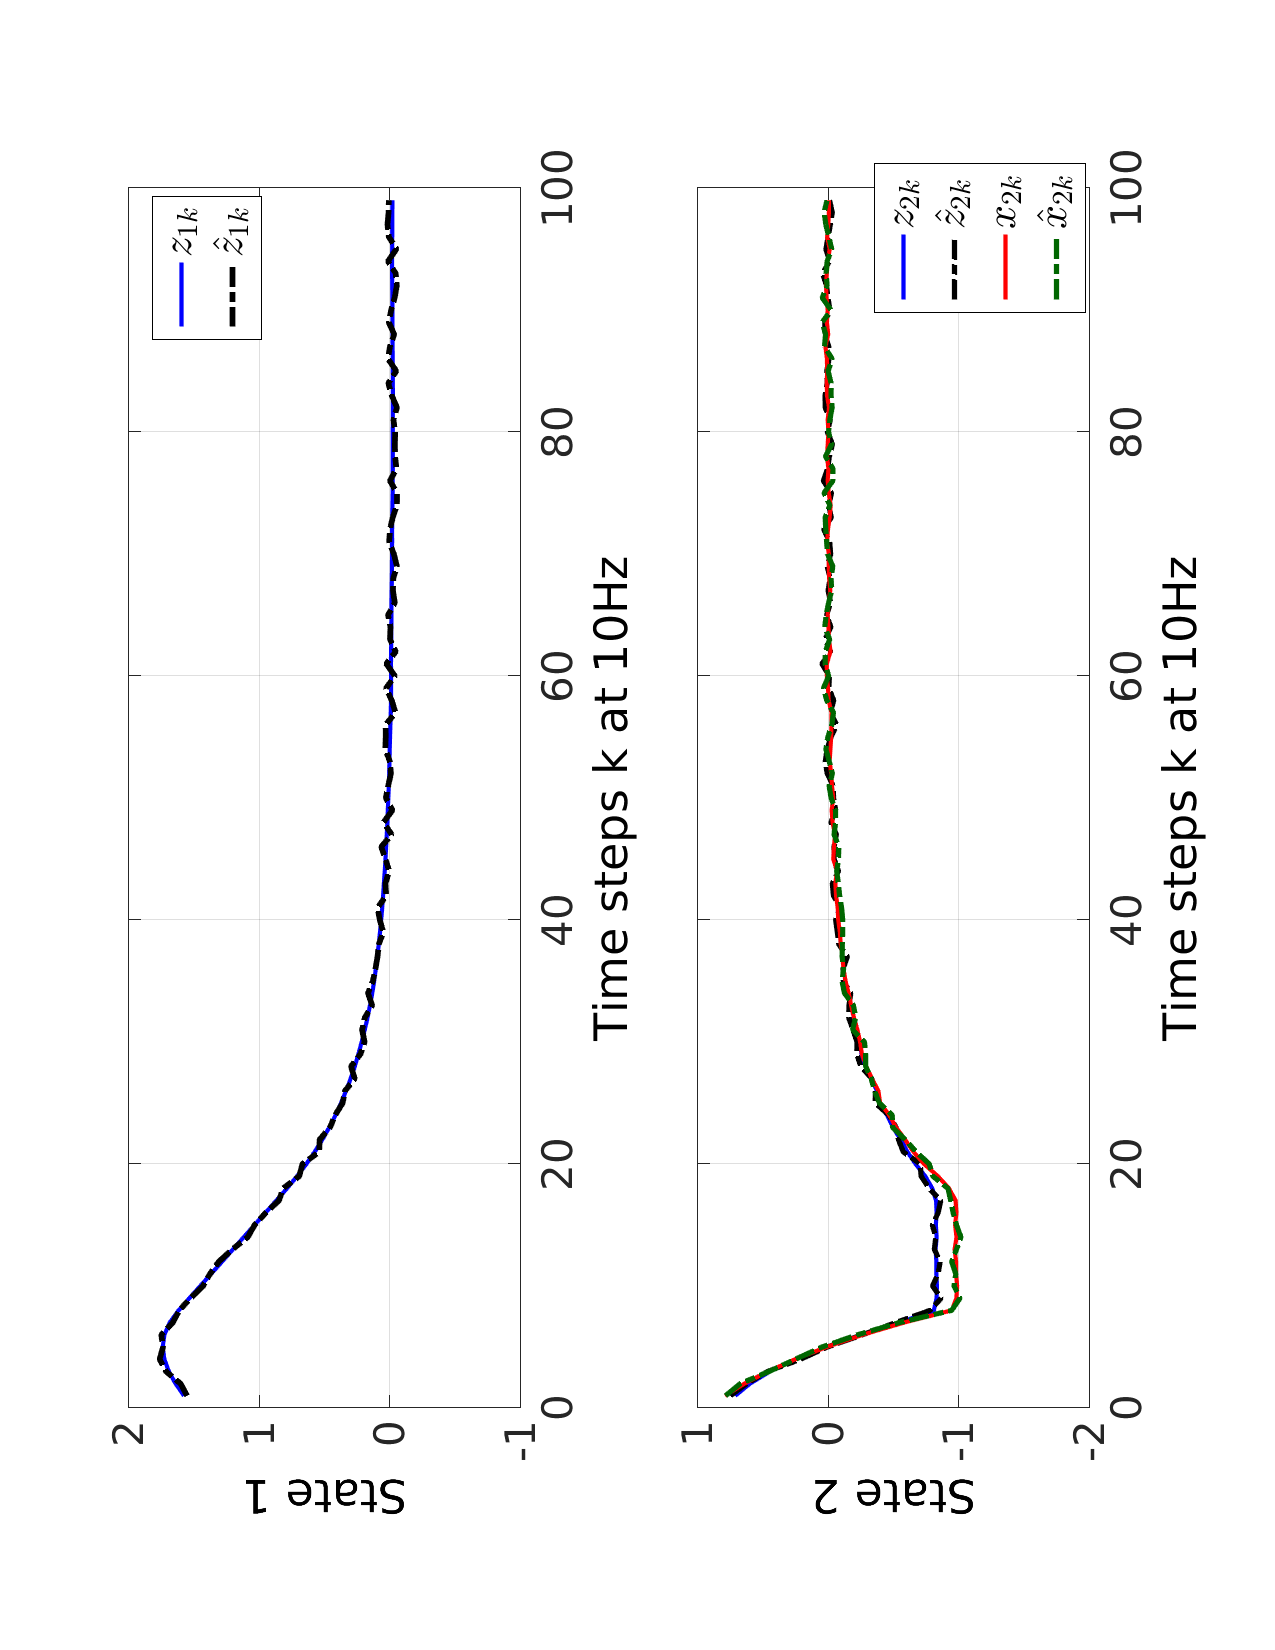
\includegraphics[angle=270,width=0.49\textwidth]{figs/AllStates_toy.pdf}
	\caption{The states and their estimates of the feedback linearized and non-linear running example. Recall that $z_1 = x_1$ therefore to reduce clutter, we only plot the first state only for the feedback linearized system. Color in online version.}
	\label{fig:AllStates_toy}
\end{figure}

For the running example of Eq. \ref{eq:toy_dynamics}, we discretize the feedback linearized system at 10Hz and formulate the controller with a horizon of $N=15$ steps. 
The cost function has parameters $Q=I$ and $R=10^{-2}$, and $W=[-10^{-2}, 10^{-2}]^2$.
The state trajectories (and estimates) for the nonlinear and linearized systems are shown in Fig. \ref{fig:AllStates_toy}.
Note that the states converge to the equilibrium 0. The input $u$ is shown in Fig. \ref{fig:input toy}, and it can be noted that $u_k \in U$ for all $k$.
%(and for the running example, $T$ preserves zero). 

\begin{figure}
	\centering	
	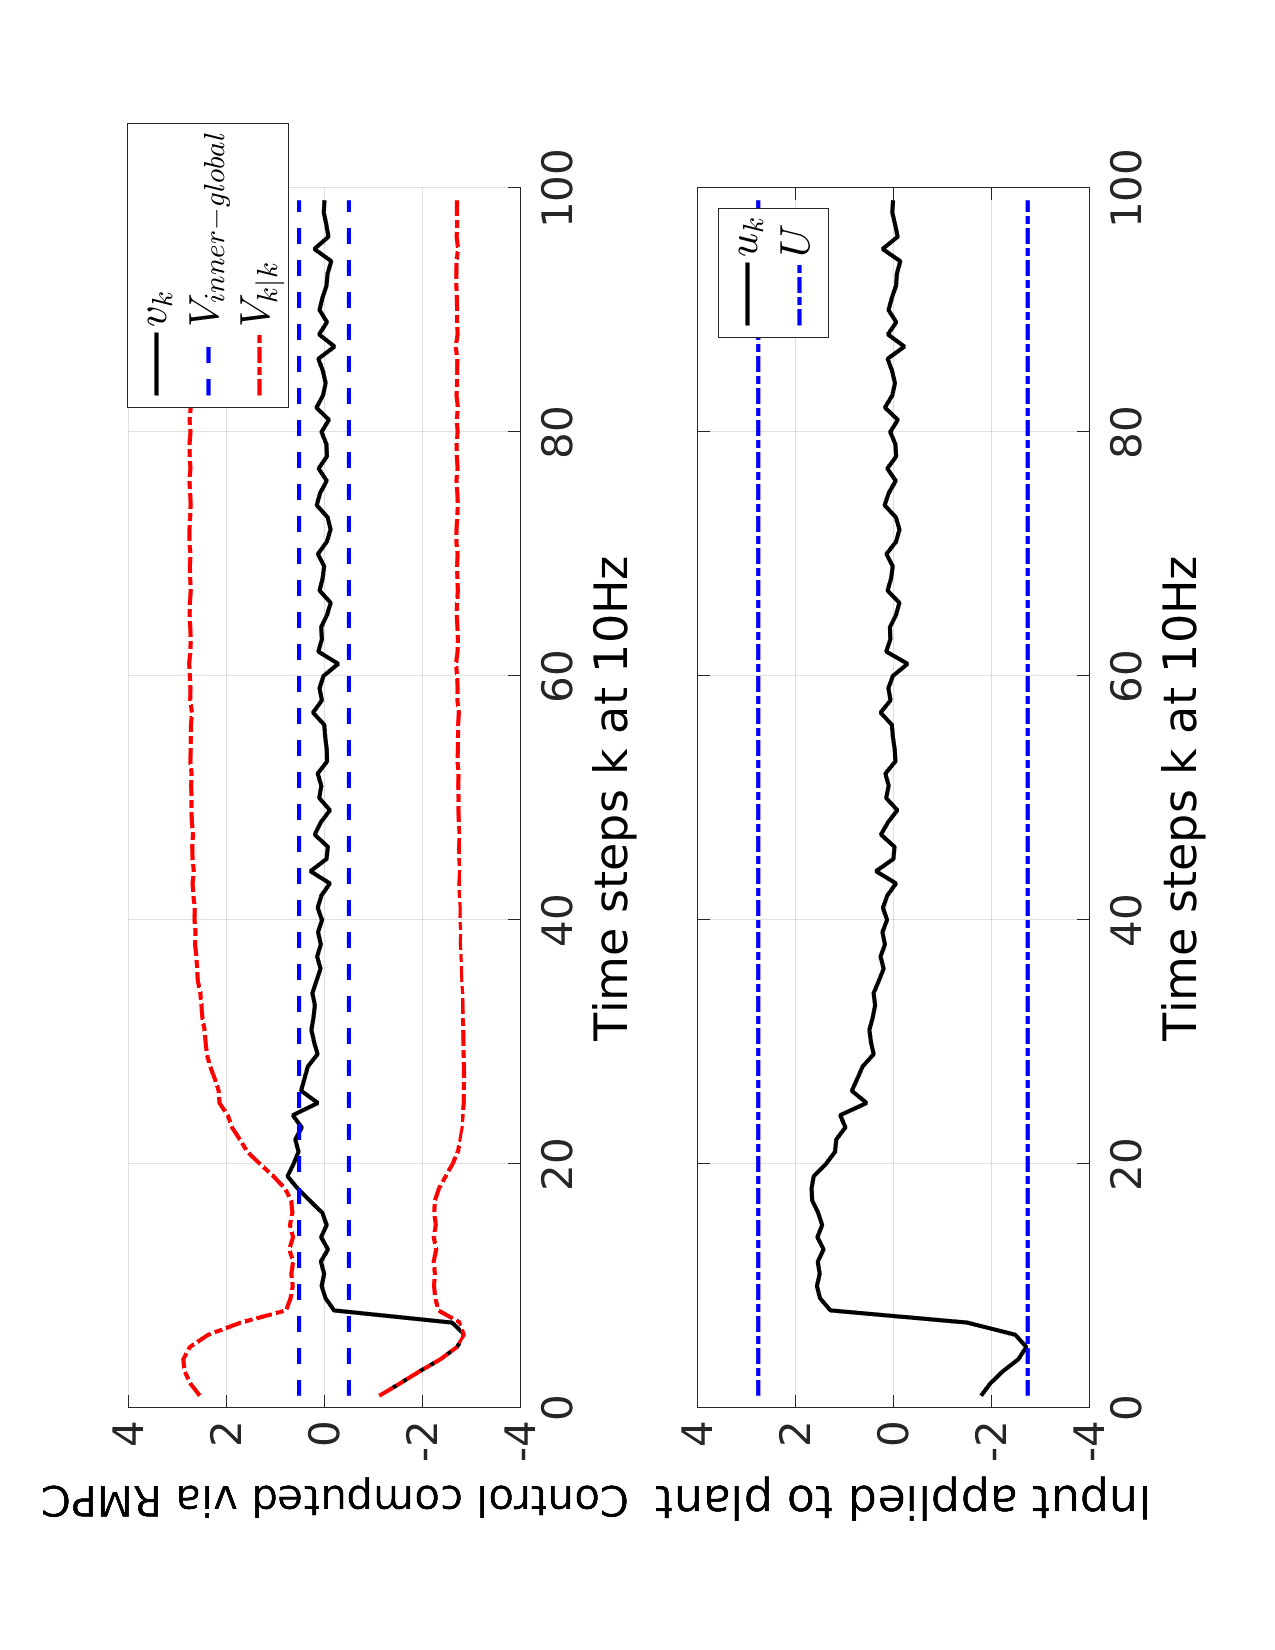
\includegraphics[angle=270,width=0.49\textwidth]{figs/u_and_v_toy.pdf}
	\caption{Inputs $v$ and $u$ and their bounds for the running example. Color in online version.}
	\label{fig:input toy}
\end{figure}




%\section*{Acknowledgements}
%We would like to thank Kuk Jang for his help in creating several of the diagrams in this paper.
\bibliographystyle{IEEEtran}%abbrv}
\bibliography{rtss2015,cdc14}

\end{document}
